% **************************************************************************************************************
% A Classic Thesis Style
% An Homage to The Elements of Typographic Style
%
% Copyright (C) 2015 André Miede http://www.miede.de
%
% If you like the style then I would appreciate a postcard. My address 
% can be found in the file ClassicThesis.pdf. A collection of the 
% postcards I received so far is available online at 
% http://postcards.miede.de
%
% License:
% This program is free software; you can redistribute it and/or modify
% it under the terms of the GNU General Public License as published by
% the Free Software Foundation; either version 2 of the License, or
% (at your option) any later version.
%
% This program is distributed in the hope that it will be useful,
% but WITHOUT ANY WARRANTY; without even the implied warranty of
% MERCHANTABILITY or FITNESS FOR A PARTICULAR PURPOSE.  See the
% GNU General Public License for more details.
%
% You should have received a copy of the GNU General Public License
% along with this program; see the file COPYING.  If not, write to
% the Free Software Foundation, Inc., 59 Temple Place - Suite 330,
% Boston, MA 02111-1307, USA.
%
% **************************************************************************************************************
\RequirePackage{fix-cm} % fix some latex issues see: http://texdoc.net/texmf-dist/doc/latex/base/fixltx2e.pdf
\documentclass[ twoside,openright,titlepage,numbers=noenddot,headinclude,%1headlines,% letterpaper a4paper
                footinclude=true,cleardoublepage=empty,abstractoff, % <--- obsolete, remove (todo)
                BCOR=5mm,paper=a4,fontsize=11pt,%11pt,a4paper,%
                ngerman,american,%
                ]{scrreprt}

%********************************************************************
% Note: Make all your adjustments in here
%*******************************************************
% ****************************************************************************************************
% classicthesis-config.tex 
% formerly known as loadpackages.sty, classicthesis-ldpkg.sty, and classicthesis-preamble.sty 
% Use it at the beginning of your ClassicThesis.tex, or as a LaTeX Preamble 
% in your ClassicThesis.{tex,lyx} with % ****************************************************************************************************
% classicthesis-config.tex 
% formerly known as loadpackages.sty, classicthesis-ldpkg.sty, and classicthesis-preamble.sty 
% Use it at the beginning of your ClassicThesis.tex, or as a LaTeX Preamble 
% in your ClassicThesis.{tex,lyx} with % ****************************************************************************************************
% classicthesis-config.tex 
% formerly known as loadpackages.sty, classicthesis-ldpkg.sty, and classicthesis-preamble.sty 
% Use it at the beginning of your ClassicThesis.tex, or as a LaTeX Preamble 
% in your ClassicThesis.{tex,lyx} with \input{classicthesis-config}
% ****************************************************************************************************  
% If you like the classicthesis, then I would appreciate a postcard. 
% My address can be found in the file ClassicThesis.pdf. A collection 
% of the postcards I received so far is available online at 
% http://postcards.miede.de
% ****************************************************************************************************


% ****************************************************************************************************
% 0. Set the encoding of your files. UTF-8 is the only sensible encoding nowadays. If you can't read
% äöüßáéçèê∂åëæƒÏ€ then change the encoding setting in your editor, not the line below. If your editor
% does not support utf8 use another editor!
% ****************************************************************************************************
\PassOptionsToPackage{utf8}{inputenc}
    \usepackage{inputenc}

% ****************************************************************************************************
% 1. Configure classicthesis for your needs here, e.g., remove "drafting" below 
% in order to deactivate the time-stamp on the pages
% ****************************************************************************************************
\PassOptionsToPackage{eulerchapternumbers,listings,%drafting,%
                      pdfspacing,floatperchapter,%linedheaders,%
                      beramono,dottedtoc,%
                      subfig,parts}{classicthesis}                                        
% ********************************************************************
% Available options for classicthesis.sty 
% (see ClassicThesis.pdf for more information):
% drafting
% parts nochapters linedheaders
% eulerchapternumbers beramono eulermath pdfspacing minionprospacing
% tocaligned dottedtoc manychapters
% listings floatperchapter subfig
% ********************************************************************


% ****************************************************************************************************
% 2. Personal data and user ad-hoc commands
% ****************************************************************************************************
\newcommand{\myTitle}{An Online Stream Processor for Timely Dataflow\xspace}
\newcommand{\myName}{Sebastian Wicki\xspace}
\newcommand{\myVersion}{version 0.1\xspace}

% ********************************************************************
% Setup, finetuning, and useful commands
% ********************************************************************
\newcounter{dummy} % necessary for correct hyperlinks (to index, bib, etc.)
\newlength{\abcd} % for ab..z string length calculation
\newcommand{\ie}{i.\,e.}
\newcommand{\Ie}{I.\,e.}
\newcommand{\eg}{e.\,g.}
\newcommand{\Eg}{E.\,g.} 
% ****************************************************************************************************


% ****************************************************************************************************
% 3. Loading some handy packages
% ****************************************************************************************************
% ********************************************************************
% Shut up warnings
% ********************************************************************
\usepackage{silence}
\WarningFilter{scrreprt}{Usage of package `titlesec'}
%\WarningFilter{scrreprt}{Activating an ugly workaround}
\WarningFilter{fixltx2e}{}
\WarningFilter{titlesec}{Non standard sectioning command detected}

% ******************************************************************** 
% Packages with options that might require adjustments
% ******************************************************************** 
%\PassOptionsToPackage{ngerman,american}{babel}   % change this to your language(s)
% Spanish languages need extra options in order to work with this template
%\PassOptionsToPackage{spanish,es-lcroman}{babel}
    \usepackage{babel}                  

\usepackage{hyphenat}
\hyphenation{que-ries data-flow time-stamp time-ly Ab-om-ona-tion Time-ly}

\newcommand\TODO[1]{%
\ifthenelse{\equal{#1}{}}%
{\textcolor{Maroon}{\textbf{TODO.}}}%
{{\color{Maroon} \textbf{TODO:} #1}}%
}

\usepackage{verbatim}

\usepackage{csquotes}
\PassOptionsToPackage{%
    %backend=biber, %instead of bibtex
    backend=bibtex8,bibencoding=ascii,%
    language=auto,%
    style=numeric-comp,%
    %style=authoryear-comp, % Author 1999, 2010
    %bibstyle=authoryear,dashed=false, % dashed: substitute rep. author with ---
    sorting=nyt, % name, year, title
    maxbibnames=10, % default: 3, et al.
    %backref=true,%
    natbib=true % natbib compatibility mode (\citep and \citet still work)
}{biblatex}
    \usepackage{biblatex}

\PassOptionsToPackage{fleqn}{amsmath}       % math environments and more by the AMS 
    \usepackage{amsmath}

% ******************************************************************** 
% General useful packages
% ******************************************************************** 
\PassOptionsToPackage{T1}{fontenc} % T2A for cyrillics
    \usepackage{fontenc}     
\usepackage{textcomp} % fix warning with missing font shapes
\usepackage{scrhack} % fix warnings when using KOMA with listings package          
\usepackage{xspace} % to get the spacing after macros right  
\usepackage{mparhack} % get marginpar right
\usepackage{fixltx2e} % fixes some LaTeX stuff --> since 2015 in the LaTeX kernel (see below)
%\usepackage[latest]{latexrelease} % will be used once available in more distributions (ISSUE #107)
\PassOptionsToPackage{printonlyused,smaller}{acronym} 
    \usepackage{acronym} % nice macros for handling all acronyms in the thesis
    %\renewcommand{\bflabel}[1]{{#1}\hfill} % fix the list of acronyms --> no longer working
    %\renewcommand*{\acsfont}[1]{\textsc{#1}} 
    \renewcommand*{\aclabelfont}[1]{\acsfont{#1}}
% ****************************************************************************************************


% ****************************************************************************************************
% 4. Setup floats: tables, (sub)figures, and captions
% ****************************************************************************************************
\usepackage{tabularx} % better tables
    \setlength{\extrarowheight}{3pt} % increase table row height
%\newcommand{\tableheadline}[1]{\multicolumn{1}{c}{\spacedlowsmallcaps{#1}}}
\newcommand{\tableheadline}[1]{\multicolumn{1}{l}{\textit{#1}}}
\newcommand{\myfloatalign}{\centering} % to be used with each float for alignment
\usepackage{caption}
% Thanks to cgnieder and Claus Lahiri
% http://tex.stackexchange.com/questions/69349/spacedlowsmallcaps-in-caption-label
% [REMOVED DUE TO OTHER PROBLEMS, SEE ISSUE #82]    
%\DeclareCaptionLabelFormat{smallcaps}{\bothIfFirst{#1}{~}\MakeTextLowercase{\textsc{#2}}}
%\captionsetup{font=small,labelformat=smallcaps} % format=hang,
\captionsetup{font=small,labelfont=it,format=plain} % format=hang,
\usepackage{subfig}  
% ****************************************************************************************************


% ****************************************************************************************************
% 5. Setup code listings
% ****************************************************************************************************
\usepackage{listings} 
%\lstset{emph={trueIndex,root},emphstyle=\color{BlueViolet}}%\underbar} % for special keywords

% Define Language
\lstdefinelanguage{Rust}
{
  % list of keywords
  morekeywords={
    abstract,alignof,as,become,box,break,const,continue,crate,do,else,enum,
        extern,false,final,fn,for,if,impl,in,let,loop,macro,match,mod,move,mut,
        offsetof,override,priv,proc,pub,pure,ref,return,Self,self,sizeof,
        static,struct,super,trait,true,type,typeof,unsafe,unsized,use,virtual,
        where,while,yield
  },
  otherkeywords={:,\.,|,=,=>,->,\#!,?},
  sensitive, % keywords are not case-sensitive
  morecomment=[l]{//}, % l is for line comment
  morecomment=[s]{/*}{*/}, % s is for start and end delimiter
  morestring=[b]" % defines that strings are enclosed in double quotes
}

\lstset{language=Rust,%C++,
    morekeywords={PassOptionsToPackage,selectlanguage},
    keywordstyle=\color{RoyalBlue},%\bfseries,
    basicstyle=\small\color{darkgray}\ttfamily,
    identifierstyle=\color{Black},
    commentstyle=\color{Gray}\ttfamily,
    stringstyle=\color{Maroon}\ttfamily,
    numbers=none,%left,%
    numberstyle=\scriptsize,%\tiny
    stepnumber=5,
    numbersep=8pt,
    showstringspaces=false,
    breaklines=true,
    %frameround=tttt,
    frame=single,
    rulecolor=\color{lstbackground},
    backgroundcolor=\color{lstbackground},
    captionpos=b,
    belowcaptionskip=.75\baselineskip,
    aboveskip=\baselineskip,
    literate={\\\-}{}{0\discretionary{-}{}{}},
} 
% ****************************************************************************************************             


% ****************************************************************************************************
% 6. PDFLaTeX, hyperreferences and citation backreferences
% ****************************************************************************************************
% ********************************************************************
% Using PDFLaTeX
% ********************************************************************
\PassOptionsToPackage{hyperfootnotes=false,pdfpagelabels}{hyperref}
    \usepackage{hyperref}  % backref linktocpage pagebackref
\pdfcompresslevel=9
\pdfadjustspacing=1 
\PassOptionsToPackage{pdftex}{graphicx}
    \usepackage{graphicx} 
 

% ********************************************************************
% Hyperreferences
% ********************************************************************
\hypersetup{%
    %draft, % = no hyperlinking at all (useful in b/w printouts)
    colorlinks=true, linktocpage=true, pdfstartpage=3, pdfstartview=FitV,%
    % uncomment the following line if you want to have black links (e.g., for printing)
    %colorlinks=false, linktocpage=false, pdfstartpage=3, pdfstartview=FitV, pdfborder={0 0 0},%
    breaklinks=true, pdfpagemode=UseNone, pageanchor=true, pdfpagemode=UseOutlines,%
    plainpages=false, bookmarksnumbered, bookmarksopen=true, bookmarksopenlevel=1,%
    hypertexnames=true, pdfhighlight=/O,%nesting=true,%frenchlinks,%
    urlcolor=webbrown, linkcolor=RoyalBlue, citecolor=webgreen, %pagecolor=RoyalBlue,%
    %urlcolor=Black, linkcolor=Black, citecolor=Black, %pagecolor=Black,%
    pdftitle={\myTitle},%
    pdfauthor={Sebastian Wicki},%
    pdfsubject={},%
    pdfkeywords={},%
    pdfcreator={pdfLaTeX},%
    pdfproducer={LaTeX with hyperref and classicthesis}%
}   

% ********************************************************************
% Setup autoreferences
% ********************************************************************
% There are some issues regarding autorefnames
% http://www.ureader.de/msg/136221647.aspx
% http://www.tex.ac.uk/cgi-bin/texfaq2html?label=latexwords
% you have to redefine the makros for the 
% language you use, e.g., american, ngerman
% (as chosen when loading babel/AtBeginDocument)
% ********************************************************************
\makeatletter
\@ifpackageloaded{babel}%
    {%
       \addto\extrasamerican{%
			\renewcommand*{\figureautorefname}{Figure}%
			\renewcommand*{\tableautorefname}{Table}%
			\renewcommand*{\partautorefname}{Part}%
			\renewcommand*{\chapterautorefname}{Chapter}%
			\renewcommand*{\sectionautorefname}{Section}%
			\renewcommand*{\subsectionautorefname}{Section}%
			\renewcommand*{\subsubsectionautorefname}{Section}%     
                }%
       \addto\extrasngerman{% 
			\renewcommand*{\paragraphautorefname}{Absatz}%
			\renewcommand*{\subparagraphautorefname}{Unterabsatz}%
			\renewcommand*{\footnoteautorefname}{Fu\"snote}%
			\renewcommand*{\FancyVerbLineautorefname}{Zeile}%
			\renewcommand*{\theoremautorefname}{Theorem}%
			\renewcommand*{\appendixautorefname}{Anhang}%
			\renewcommand*{\equationautorefname}{Gleichung}%        
			\renewcommand*{\itemautorefname}{Punkt}%
                }%  
            % Fix to getting autorefs for subfigures right (thanks to Belinda Vogt for changing the definition)
            \providecommand{\subfigureautorefname}{\figureautorefname}%             
    }{\relax}
\makeatother


% ****************************************************************************************************
% 7. Last calls before the bar closes
% ****************************************************************************************************
% ********************************************************************
% Development Stuff
% ********************************************************************
%\listfiles
%\PassOptionsToPackage{l2tabu,orthodox,abort}{nag}
%   \usepackage{nag}
%\PassOptionsToPackage{warning, all}{onlyamsmath}
%   \usepackage{onlyamsmath}

% ********************************************************************
% Last, but not least...
% ********************************************************************
\usepackage{classicthesis} 
% ****************************************************************************************************

% ****************************************************************************************************
% 8. Further adjustments (experimental)
% ****************************************************************************************************
% ********************************************************************
% Changing the text area
% ********************************************************************
%\linespread{1.05} % a bit more for Palatino
%\areaset[current]{312pt}{761pt} % 686 (factor 2.2) + 33 head + 42 head \the\footskip
%\setlength{\marginparwidth}{7em}%
%\setlength{\marginparsep}{2em}%

% ********************************************************************
% Using different fonts
% ********************************************************************
%\usepackage[oldstylenums]{kpfonts} % oldstyle notextcomp
%\usepackage[osf]{libertine}
%\usepackage[light,condensed,math]{iwona}
%\renewcommand{\sfdefault}{iwona}
%\usepackage{lmodern} % <-- no osf support :-(
%\usepackage{cfr-lm} % 
%\usepackage[urw-garamond]{mathdesign} <-- no osf support :-(
%\usepackage[default,osfigures]{opensans} % scale=0.95 
%\usepackage[sfdefault]{FiraSans}

% ****************************************************************************************************

% ********************************************************************
% Systems Group title page
% ********************************************************************
\usepackage[masterthesis]{systems-cover/systems-cover}
\covernum{155}
\covertitle{\myTitle}
\coverauthor{\myName}
\coversupervisedby{Dr.\ Desislava Dimitrova \\ Dr.\ John Liagouris \\ Prof.\ Timothy Roscoe}
\coverdate{May 2016 -- November 2016}

% ********************************************************************
% Track changes
% ********************************************************************
\usepackage[xcolor]{changebar}

\newcommand{\cbdefaultcolor}{BurntOrange}

\cbcolor{\cbdefaultcolor}

\newenvironment{addedbar}%
{\cbcolor{YellowGreen}\begin{changebar}}%
{\end{changebar}\cbcolor{\cbdefaultcolor}}

% References
\newcommand*{\fullref}[1]{\hyperref[{#1}]{\ref*{#1} \nameref*{#1}}}

% New chapters at even page
%\renewcommand{\cleardoublepage}{\cleardoubleevenemptypage}
% ********************************************************************
% For the Declaration of Originality
% ********************************************************************
\usepackage{pdfpages}

% ****************************************************************************************************  
% If you like the classicthesis, then I would appreciate a postcard. 
% My address can be found in the file ClassicThesis.pdf. A collection 
% of the postcards I received so far is available online at 
% http://postcards.miede.de
% ****************************************************************************************************


% ****************************************************************************************************
% 0. Set the encoding of your files. UTF-8 is the only sensible encoding nowadays. If you can't read
% äöüßáéçèê∂åëæƒÏ€ then change the encoding setting in your editor, not the line below. If your editor
% does not support utf8 use another editor!
% ****************************************************************************************************
\PassOptionsToPackage{utf8}{inputenc}
    \usepackage{inputenc}

% ****************************************************************************************************
% 1. Configure classicthesis for your needs here, e.g., remove "drafting" below 
% in order to deactivate the time-stamp on the pages
% ****************************************************************************************************
\PassOptionsToPackage{eulerchapternumbers,listings,%drafting,%
                      pdfspacing,floatperchapter,%linedheaders,%
                      beramono,dottedtoc,%
                      subfig,parts}{classicthesis}                                        
% ********************************************************************
% Available options for classicthesis.sty 
% (see ClassicThesis.pdf for more information):
% drafting
% parts nochapters linedheaders
% eulerchapternumbers beramono eulermath pdfspacing minionprospacing
% tocaligned dottedtoc manychapters
% listings floatperchapter subfig
% ********************************************************************


% ****************************************************************************************************
% 2. Personal data and user ad-hoc commands
% ****************************************************************************************************
\newcommand{\myTitle}{An Online Stream Processor for Timely Dataflow\xspace}
\newcommand{\myName}{Sebastian Wicki\xspace}
\newcommand{\myVersion}{version 0.1\xspace}

% ********************************************************************
% Setup, finetuning, and useful commands
% ********************************************************************
\newcounter{dummy} % necessary for correct hyperlinks (to index, bib, etc.)
\newlength{\abcd} % for ab..z string length calculation
\newcommand{\ie}{i.\,e.}
\newcommand{\Ie}{I.\,e.}
\newcommand{\eg}{e.\,g.}
\newcommand{\Eg}{E.\,g.} 
% ****************************************************************************************************


% ****************************************************************************************************
% 3. Loading some handy packages
% ****************************************************************************************************
% ********************************************************************
% Shut up warnings
% ********************************************************************
\usepackage{silence}
\WarningFilter{scrreprt}{Usage of package `titlesec'}
%\WarningFilter{scrreprt}{Activating an ugly workaround}
\WarningFilter{fixltx2e}{}
\WarningFilter{titlesec}{Non standard sectioning command detected}

% ******************************************************************** 
% Packages with options that might require adjustments
% ******************************************************************** 
%\PassOptionsToPackage{ngerman,american}{babel}   % change this to your language(s)
% Spanish languages need extra options in order to work with this template
%\PassOptionsToPackage{spanish,es-lcroman}{babel}
    \usepackage{babel}                  

\usepackage{hyphenat}
\hyphenation{que-ries data-flow time-stamp time-ly Ab-om-ona-tion Time-ly}

\newcommand\TODO[1]{%
\ifthenelse{\equal{#1}{}}%
{\textcolor{Maroon}{\textbf{TODO.}}}%
{{\color{Maroon} \textbf{TODO:} #1}}%
}

\usepackage{verbatim}

\usepackage{csquotes}
\PassOptionsToPackage{%
    %backend=biber, %instead of bibtex
    backend=bibtex8,bibencoding=ascii,%
    language=auto,%
    style=numeric-comp,%
    %style=authoryear-comp, % Author 1999, 2010
    %bibstyle=authoryear,dashed=false, % dashed: substitute rep. author with ---
    sorting=nyt, % name, year, title
    maxbibnames=10, % default: 3, et al.
    %backref=true,%
    natbib=true % natbib compatibility mode (\citep and \citet still work)
}{biblatex}
    \usepackage{biblatex}

\PassOptionsToPackage{fleqn}{amsmath}       % math environments and more by the AMS 
    \usepackage{amsmath}

% ******************************************************************** 
% General useful packages
% ******************************************************************** 
\PassOptionsToPackage{T1}{fontenc} % T2A for cyrillics
    \usepackage{fontenc}     
\usepackage{textcomp} % fix warning with missing font shapes
\usepackage{scrhack} % fix warnings when using KOMA with listings package          
\usepackage{xspace} % to get the spacing after macros right  
\usepackage{mparhack} % get marginpar right
\usepackage{fixltx2e} % fixes some LaTeX stuff --> since 2015 in the LaTeX kernel (see below)
%\usepackage[latest]{latexrelease} % will be used once available in more distributions (ISSUE #107)
\PassOptionsToPackage{printonlyused,smaller}{acronym} 
    \usepackage{acronym} % nice macros for handling all acronyms in the thesis
    %\renewcommand{\bflabel}[1]{{#1}\hfill} % fix the list of acronyms --> no longer working
    %\renewcommand*{\acsfont}[1]{\textsc{#1}} 
    \renewcommand*{\aclabelfont}[1]{\acsfont{#1}}
% ****************************************************************************************************


% ****************************************************************************************************
% 4. Setup floats: tables, (sub)figures, and captions
% ****************************************************************************************************
\usepackage{tabularx} % better tables
    \setlength{\extrarowheight}{3pt} % increase table row height
%\newcommand{\tableheadline}[1]{\multicolumn{1}{c}{\spacedlowsmallcaps{#1}}}
\newcommand{\tableheadline}[1]{\multicolumn{1}{l}{\textit{#1}}}
\newcommand{\myfloatalign}{\centering} % to be used with each float for alignment
\usepackage{caption}
% Thanks to cgnieder and Claus Lahiri
% http://tex.stackexchange.com/questions/69349/spacedlowsmallcaps-in-caption-label
% [REMOVED DUE TO OTHER PROBLEMS, SEE ISSUE #82]    
%\DeclareCaptionLabelFormat{smallcaps}{\bothIfFirst{#1}{~}\MakeTextLowercase{\textsc{#2}}}
%\captionsetup{font=small,labelformat=smallcaps} % format=hang,
\captionsetup{font=small,labelfont=it,format=plain} % format=hang,
\usepackage{subfig}  
% ****************************************************************************************************


% ****************************************************************************************************
% 5. Setup code listings
% ****************************************************************************************************
\usepackage{listings} 
%\lstset{emph={trueIndex,root},emphstyle=\color{BlueViolet}}%\underbar} % for special keywords

% Define Language
\lstdefinelanguage{Rust}
{
  % list of keywords
  morekeywords={
    abstract,alignof,as,become,box,break,const,continue,crate,do,else,enum,
        extern,false,final,fn,for,if,impl,in,let,loop,macro,match,mod,move,mut,
        offsetof,override,priv,proc,pub,pure,ref,return,Self,self,sizeof,
        static,struct,super,trait,true,type,typeof,unsafe,unsized,use,virtual,
        where,while,yield
  },
  otherkeywords={:,\.,|,=,=>,->,\#!,?},
  sensitive, % keywords are not case-sensitive
  morecomment=[l]{//}, % l is for line comment
  morecomment=[s]{/*}{*/}, % s is for start and end delimiter
  morestring=[b]" % defines that strings are enclosed in double quotes
}

\lstset{language=Rust,%C++,
    morekeywords={PassOptionsToPackage,selectlanguage},
    keywordstyle=\color{RoyalBlue},%\bfseries,
    basicstyle=\small\color{darkgray}\ttfamily,
    identifierstyle=\color{Black},
    commentstyle=\color{Gray}\ttfamily,
    stringstyle=\color{Maroon}\ttfamily,
    numbers=none,%left,%
    numberstyle=\scriptsize,%\tiny
    stepnumber=5,
    numbersep=8pt,
    showstringspaces=false,
    breaklines=true,
    %frameround=tttt,
    frame=single,
    rulecolor=\color{lstbackground},
    backgroundcolor=\color{lstbackground},
    captionpos=b,
    belowcaptionskip=.75\baselineskip,
    aboveskip=\baselineskip,
    literate={\\\-}{}{0\discretionary{-}{}{}},
} 
% ****************************************************************************************************             


% ****************************************************************************************************
% 6. PDFLaTeX, hyperreferences and citation backreferences
% ****************************************************************************************************
% ********************************************************************
% Using PDFLaTeX
% ********************************************************************
\PassOptionsToPackage{hyperfootnotes=false,pdfpagelabels}{hyperref}
    \usepackage{hyperref}  % backref linktocpage pagebackref
\pdfcompresslevel=9
\pdfadjustspacing=1 
\PassOptionsToPackage{pdftex}{graphicx}
    \usepackage{graphicx} 
 

% ********************************************************************
% Hyperreferences
% ********************************************************************
\hypersetup{%
    %draft, % = no hyperlinking at all (useful in b/w printouts)
    colorlinks=true, linktocpage=true, pdfstartpage=3, pdfstartview=FitV,%
    % uncomment the following line if you want to have black links (e.g., for printing)
    %colorlinks=false, linktocpage=false, pdfstartpage=3, pdfstartview=FitV, pdfborder={0 0 0},%
    breaklinks=true, pdfpagemode=UseNone, pageanchor=true, pdfpagemode=UseOutlines,%
    plainpages=false, bookmarksnumbered, bookmarksopen=true, bookmarksopenlevel=1,%
    hypertexnames=true, pdfhighlight=/O,%nesting=true,%frenchlinks,%
    urlcolor=webbrown, linkcolor=RoyalBlue, citecolor=webgreen, %pagecolor=RoyalBlue,%
    %urlcolor=Black, linkcolor=Black, citecolor=Black, %pagecolor=Black,%
    pdftitle={\myTitle},%
    pdfauthor={Sebastian Wicki},%
    pdfsubject={},%
    pdfkeywords={},%
    pdfcreator={pdfLaTeX},%
    pdfproducer={LaTeX with hyperref and classicthesis}%
}   

% ********************************************************************
% Setup autoreferences
% ********************************************************************
% There are some issues regarding autorefnames
% http://www.ureader.de/msg/136221647.aspx
% http://www.tex.ac.uk/cgi-bin/texfaq2html?label=latexwords
% you have to redefine the makros for the 
% language you use, e.g., american, ngerman
% (as chosen when loading babel/AtBeginDocument)
% ********************************************************************
\makeatletter
\@ifpackageloaded{babel}%
    {%
       \addto\extrasamerican{%
			\renewcommand*{\figureautorefname}{Figure}%
			\renewcommand*{\tableautorefname}{Table}%
			\renewcommand*{\partautorefname}{Part}%
			\renewcommand*{\chapterautorefname}{Chapter}%
			\renewcommand*{\sectionautorefname}{Section}%
			\renewcommand*{\subsectionautorefname}{Section}%
			\renewcommand*{\subsubsectionautorefname}{Section}%     
                }%
       \addto\extrasngerman{% 
			\renewcommand*{\paragraphautorefname}{Absatz}%
			\renewcommand*{\subparagraphautorefname}{Unterabsatz}%
			\renewcommand*{\footnoteautorefname}{Fu\"snote}%
			\renewcommand*{\FancyVerbLineautorefname}{Zeile}%
			\renewcommand*{\theoremautorefname}{Theorem}%
			\renewcommand*{\appendixautorefname}{Anhang}%
			\renewcommand*{\equationautorefname}{Gleichung}%        
			\renewcommand*{\itemautorefname}{Punkt}%
                }%  
            % Fix to getting autorefs for subfigures right (thanks to Belinda Vogt for changing the definition)
            \providecommand{\subfigureautorefname}{\figureautorefname}%             
    }{\relax}
\makeatother


% ****************************************************************************************************
% 7. Last calls before the bar closes
% ****************************************************************************************************
% ********************************************************************
% Development Stuff
% ********************************************************************
%\listfiles
%\PassOptionsToPackage{l2tabu,orthodox,abort}{nag}
%   \usepackage{nag}
%\PassOptionsToPackage{warning, all}{onlyamsmath}
%   \usepackage{onlyamsmath}

% ********************************************************************
% Last, but not least...
% ********************************************************************
\usepackage{classicthesis} 
% ****************************************************************************************************

% ****************************************************************************************************
% 8. Further adjustments (experimental)
% ****************************************************************************************************
% ********************************************************************
% Changing the text area
% ********************************************************************
%\linespread{1.05} % a bit more for Palatino
%\areaset[current]{312pt}{761pt} % 686 (factor 2.2) + 33 head + 42 head \the\footskip
%\setlength{\marginparwidth}{7em}%
%\setlength{\marginparsep}{2em}%

% ********************************************************************
% Using different fonts
% ********************************************************************
%\usepackage[oldstylenums]{kpfonts} % oldstyle notextcomp
%\usepackage[osf]{libertine}
%\usepackage[light,condensed,math]{iwona}
%\renewcommand{\sfdefault}{iwona}
%\usepackage{lmodern} % <-- no osf support :-(
%\usepackage{cfr-lm} % 
%\usepackage[urw-garamond]{mathdesign} <-- no osf support :-(
%\usepackage[default,osfigures]{opensans} % scale=0.95 
%\usepackage[sfdefault]{FiraSans}

% ****************************************************************************************************

% ********************************************************************
% Systems Group title page
% ********************************************************************
\usepackage[masterthesis]{systems-cover/systems-cover}
\covernum{155}
\covertitle{\myTitle}
\coverauthor{\myName}
\coversupervisedby{Dr.\ Desislava Dimitrova \\ Dr.\ John Liagouris \\ Prof.\ Timothy Roscoe}
\coverdate{May 2016 -- November 2016}

% ********************************************************************
% Track changes
% ********************************************************************
\usepackage[xcolor]{changebar}

\newcommand{\cbdefaultcolor}{BurntOrange}

\cbcolor{\cbdefaultcolor}

\newenvironment{addedbar}%
{\cbcolor{YellowGreen}\begin{changebar}}%
{\end{changebar}\cbcolor{\cbdefaultcolor}}

% References
\newcommand*{\fullref}[1]{\hyperref[{#1}]{\ref*{#1} \nameref*{#1}}}

% New chapters at even page
%\renewcommand{\cleardoublepage}{\cleardoubleevenemptypage}
% ********************************************************************
% For the Declaration of Originality
% ********************************************************************
\usepackage{pdfpages}

% ****************************************************************************************************  
% If you like the classicthesis, then I would appreciate a postcard. 
% My address can be found in the file ClassicThesis.pdf. A collection 
% of the postcards I received so far is available online at 
% http://postcards.miede.de
% ****************************************************************************************************


% ****************************************************************************************************
% 0. Set the encoding of your files. UTF-8 is the only sensible encoding nowadays. If you can't read
% äöüßáéçèê∂åëæƒÏ€ then change the encoding setting in your editor, not the line below. If your editor
% does not support utf8 use another editor!
% ****************************************************************************************************
\PassOptionsToPackage{utf8}{inputenc}
    \usepackage{inputenc}

% ****************************************************************************************************
% 1. Configure classicthesis for your needs here, e.g., remove "drafting" below 
% in order to deactivate the time-stamp on the pages
% ****************************************************************************************************
\PassOptionsToPackage{eulerchapternumbers,listings,%drafting,%
                      pdfspacing,floatperchapter,%linedheaders,%
                      beramono,dottedtoc,%
                      subfig,parts}{classicthesis}                                        
% ********************************************************************
% Available options for classicthesis.sty 
% (see ClassicThesis.pdf for more information):
% drafting
% parts nochapters linedheaders
% eulerchapternumbers beramono eulermath pdfspacing minionprospacing
% tocaligned dottedtoc manychapters
% listings floatperchapter subfig
% ********************************************************************


% ****************************************************************************************************
% 2. Personal data and user ad-hoc commands
% ****************************************************************************************************
\newcommand{\myTitle}{An Online Stream Processor for Timely Dataflow\xspace}
\newcommand{\myName}{Sebastian Wicki\xspace}
\newcommand{\myVersion}{version 0.1\xspace}

% ********************************************************************
% Setup, finetuning, and useful commands
% ********************************************************************
\newcounter{dummy} % necessary for correct hyperlinks (to index, bib, etc.)
\newlength{\abcd} % for ab..z string length calculation
\newcommand{\ie}{i.\,e.}
\newcommand{\Ie}{I.\,e.}
\newcommand{\eg}{e.\,g.}
\newcommand{\Eg}{E.\,g.} 
% ****************************************************************************************************


% ****************************************************************************************************
% 3. Loading some handy packages
% ****************************************************************************************************
% ********************************************************************
% Shut up warnings
% ********************************************************************
\usepackage{silence}
\WarningFilter{scrreprt}{Usage of package `titlesec'}
%\WarningFilter{scrreprt}{Activating an ugly workaround}
\WarningFilter{fixltx2e}{}
\WarningFilter{titlesec}{Non standard sectioning command detected}

% ******************************************************************** 
% Packages with options that might require adjustments
% ******************************************************************** 
%\PassOptionsToPackage{ngerman,american}{babel}   % change this to your language(s)
% Spanish languages need extra options in order to work with this template
%\PassOptionsToPackage{spanish,es-lcroman}{babel}
    \usepackage{babel}                  

\usepackage{hyphenat}
\hyphenation{que-ries data-flow time-stamp time-ly Ab-om-ona-tion Time-ly}

\newcommand\TODO[1]{%
\ifthenelse{\equal{#1}{}}%
{\textcolor{Maroon}{\textbf{TODO.}}}%
{{\color{Maroon} \textbf{TODO:} #1}}%
}

\usepackage{verbatim}

\usepackage{csquotes}
\PassOptionsToPackage{%
    %backend=biber, %instead of bibtex
    backend=bibtex8,bibencoding=ascii,%
    language=auto,%
    style=numeric-comp,%
    %style=authoryear-comp, % Author 1999, 2010
    %bibstyle=authoryear,dashed=false, % dashed: substitute rep. author with ---
    sorting=nyt, % name, year, title
    maxbibnames=10, % default: 3, et al.
    %backref=true,%
    natbib=true % natbib compatibility mode (\citep and \citet still work)
}{biblatex}
    \usepackage{biblatex}

\PassOptionsToPackage{fleqn}{amsmath}       % math environments and more by the AMS 
    \usepackage{amsmath}

% ******************************************************************** 
% General useful packages
% ******************************************************************** 
\PassOptionsToPackage{T1}{fontenc} % T2A for cyrillics
    \usepackage{fontenc}     
\usepackage{textcomp} % fix warning with missing font shapes
\usepackage{scrhack} % fix warnings when using KOMA with listings package          
\usepackage{xspace} % to get the spacing after macros right  
\usepackage{mparhack} % get marginpar right
\usepackage{fixltx2e} % fixes some LaTeX stuff --> since 2015 in the LaTeX kernel (see below)
%\usepackage[latest]{latexrelease} % will be used once available in more distributions (ISSUE #107)
\PassOptionsToPackage{printonlyused,smaller}{acronym} 
    \usepackage{acronym} % nice macros for handling all acronyms in the thesis
    %\renewcommand{\bflabel}[1]{{#1}\hfill} % fix the list of acronyms --> no longer working
    %\renewcommand*{\acsfont}[1]{\textsc{#1}} 
    \renewcommand*{\aclabelfont}[1]{\acsfont{#1}}
% ****************************************************************************************************


% ****************************************************************************************************
% 4. Setup floats: tables, (sub)figures, and captions
% ****************************************************************************************************
\usepackage{tabularx} % better tables
    \setlength{\extrarowheight}{3pt} % increase table row height
%\newcommand{\tableheadline}[1]{\multicolumn{1}{c}{\spacedlowsmallcaps{#1}}}
\newcommand{\tableheadline}[1]{\multicolumn{1}{l}{\textit{#1}}}
\newcommand{\myfloatalign}{\centering} % to be used with each float for alignment
\usepackage{caption}
% Thanks to cgnieder and Claus Lahiri
% http://tex.stackexchange.com/questions/69349/spacedlowsmallcaps-in-caption-label
% [REMOVED DUE TO OTHER PROBLEMS, SEE ISSUE #82]    
%\DeclareCaptionLabelFormat{smallcaps}{\bothIfFirst{#1}{~}\MakeTextLowercase{\textsc{#2}}}
%\captionsetup{font=small,labelformat=smallcaps} % format=hang,
\captionsetup{font=small,labelfont=it,format=plain} % format=hang,
\usepackage{subfig}  
% ****************************************************************************************************


% ****************************************************************************************************
% 5. Setup code listings
% ****************************************************************************************************
\usepackage{listings} 
%\lstset{emph={trueIndex,root},emphstyle=\color{BlueViolet}}%\underbar} % for special keywords

% Define Language
\lstdefinelanguage{Rust}
{
  % list of keywords
  morekeywords={
    abstract,alignof,as,become,box,break,const,continue,crate,do,else,enum,
        extern,false,final,fn,for,if,impl,in,let,loop,macro,match,mod,move,mut,
        offsetof,override,priv,proc,pub,pure,ref,return,Self,self,sizeof,
        static,struct,super,trait,true,type,typeof,unsafe,unsized,use,virtual,
        where,while,yield
  },
  otherkeywords={:,\.,|,=,=>,->,\#!,?},
  sensitive, % keywords are not case-sensitive
  morecomment=[l]{//}, % l is for line comment
  morecomment=[s]{/*}{*/}, % s is for start and end delimiter
  morestring=[b]" % defines that strings are enclosed in double quotes
}

\lstset{language=Rust,%C++,
    morekeywords={PassOptionsToPackage,selectlanguage},
    keywordstyle=\color{RoyalBlue},%\bfseries,
    basicstyle=\small\color{darkgray}\ttfamily,
    identifierstyle=\color{Black},
    commentstyle=\color{Gray}\ttfamily,
    stringstyle=\color{Maroon}\ttfamily,
    numbers=none,%left,%
    numberstyle=\scriptsize,%\tiny
    stepnumber=5,
    numbersep=8pt,
    showstringspaces=false,
    breaklines=true,
    %frameround=tttt,
    frame=single,
    rulecolor=\color{lstbackground},
    backgroundcolor=\color{lstbackground},
    captionpos=b,
    belowcaptionskip=.75\baselineskip,
    aboveskip=\baselineskip,
    literate={\\\-}{}{0\discretionary{-}{}{}},
} 
% ****************************************************************************************************             


% ****************************************************************************************************
% 6. PDFLaTeX, hyperreferences and citation backreferences
% ****************************************************************************************************
% ********************************************************************
% Using PDFLaTeX
% ********************************************************************
\PassOptionsToPackage{hyperfootnotes=false,pdfpagelabels}{hyperref}
    \usepackage{hyperref}  % backref linktocpage pagebackref
\pdfcompresslevel=9
\pdfadjustspacing=1 
\PassOptionsToPackage{pdftex}{graphicx}
    \usepackage{graphicx} 
 

% ********************************************************************
% Hyperreferences
% ********************************************************************
\hypersetup{%
    %draft, % = no hyperlinking at all (useful in b/w printouts)
    colorlinks=true, linktocpage=true, pdfstartpage=3, pdfstartview=FitV,%
    % uncomment the following line if you want to have black links (e.g., for printing)
    %colorlinks=false, linktocpage=false, pdfstartpage=3, pdfstartview=FitV, pdfborder={0 0 0},%
    breaklinks=true, pdfpagemode=UseNone, pageanchor=true, pdfpagemode=UseOutlines,%
    plainpages=false, bookmarksnumbered, bookmarksopen=true, bookmarksopenlevel=1,%
    hypertexnames=true, pdfhighlight=/O,%nesting=true,%frenchlinks,%
    urlcolor=webbrown, linkcolor=RoyalBlue, citecolor=webgreen, %pagecolor=RoyalBlue,%
    %urlcolor=Black, linkcolor=Black, citecolor=Black, %pagecolor=Black,%
    pdftitle={\myTitle},%
    pdfauthor={Sebastian Wicki},%
    pdfsubject={},%
    pdfkeywords={},%
    pdfcreator={pdfLaTeX},%
    pdfproducer={LaTeX with hyperref and classicthesis}%
}   

% ********************************************************************
% Setup autoreferences
% ********************************************************************
% There are some issues regarding autorefnames
% http://www.ureader.de/msg/136221647.aspx
% http://www.tex.ac.uk/cgi-bin/texfaq2html?label=latexwords
% you have to redefine the makros for the 
% language you use, e.g., american, ngerman
% (as chosen when loading babel/AtBeginDocument)
% ********************************************************************
\makeatletter
\@ifpackageloaded{babel}%
    {%
       \addto\extrasamerican{%
			\renewcommand*{\figureautorefname}{Figure}%
			\renewcommand*{\tableautorefname}{Table}%
			\renewcommand*{\partautorefname}{Part}%
			\renewcommand*{\chapterautorefname}{Chapter}%
			\renewcommand*{\sectionautorefname}{Section}%
			\renewcommand*{\subsectionautorefname}{Section}%
			\renewcommand*{\subsubsectionautorefname}{Section}%     
                }%
       \addto\extrasngerman{% 
			\renewcommand*{\paragraphautorefname}{Absatz}%
			\renewcommand*{\subparagraphautorefname}{Unterabsatz}%
			\renewcommand*{\footnoteautorefname}{Fu\"snote}%
			\renewcommand*{\FancyVerbLineautorefname}{Zeile}%
			\renewcommand*{\theoremautorefname}{Theorem}%
			\renewcommand*{\appendixautorefname}{Anhang}%
			\renewcommand*{\equationautorefname}{Gleichung}%        
			\renewcommand*{\itemautorefname}{Punkt}%
                }%  
            % Fix to getting autorefs for subfigures right (thanks to Belinda Vogt for changing the definition)
            \providecommand{\subfigureautorefname}{\figureautorefname}%             
    }{\relax}
\makeatother


% ****************************************************************************************************
% 7. Last calls before the bar closes
% ****************************************************************************************************
% ********************************************************************
% Development Stuff
% ********************************************************************
%\listfiles
%\PassOptionsToPackage{l2tabu,orthodox,abort}{nag}
%   \usepackage{nag}
%\PassOptionsToPackage{warning, all}{onlyamsmath}
%   \usepackage{onlyamsmath}

% ********************************************************************
% Last, but not least...
% ********************************************************************
\usepackage{classicthesis} 
% ****************************************************************************************************

% ****************************************************************************************************
% 8. Further adjustments (experimental)
% ****************************************************************************************************
% ********************************************************************
% Changing the text area
% ********************************************************************
%\linespread{1.05} % a bit more for Palatino
%\areaset[current]{312pt}{761pt} % 686 (factor 2.2) + 33 head + 42 head \the\footskip
%\setlength{\marginparwidth}{7em}%
%\setlength{\marginparsep}{2em}%

% ********************************************************************
% Using different fonts
% ********************************************************************
%\usepackage[oldstylenums]{kpfonts} % oldstyle notextcomp
%\usepackage[osf]{libertine}
%\usepackage[light,condensed,math]{iwona}
%\renewcommand{\sfdefault}{iwona}
%\usepackage{lmodern} % <-- no osf support :-(
%\usepackage{cfr-lm} % 
%\usepackage[urw-garamond]{mathdesign} <-- no osf support :-(
%\usepackage[default,osfigures]{opensans} % scale=0.95 
%\usepackage[sfdefault]{FiraSans}

% ****************************************************************************************************

% ********************************************************************
% Systems Group title page
% ********************************************************************
\usepackage[masterthesis]{systems-cover/systems-cover}
\covernum{155}
\covertitle{\myTitle}
\coverauthor{\myName}
\coversupervisedby{Dr.\ Desislava Dimitrova \\ Dr.\ John Liagouris \\ Prof.\ Timothy Roscoe}
\coverdate{May 2016 -- November 2016}

% ********************************************************************
% Track changes
% ********************************************************************
\usepackage[xcolor]{changebar}

\newcommand{\cbdefaultcolor}{BurntOrange}

\cbcolor{\cbdefaultcolor}

\newenvironment{addedbar}%
{\cbcolor{YellowGreen}\begin{changebar}}%
{\end{changebar}\cbcolor{\cbdefaultcolor}}

% References
\newcommand*{\fullref}[1]{\hyperref[{#1}]{\ref*{#1} \nameref*{#1}}}

% New chapters at even page
%\renewcommand{\cleardoublepage}{\cleardoubleevenemptypage}
% ********************************************************************
% For the Declaration of Originality
% ********************************************************************
\usepackage{pdfpages}


%********************************************************************
% Bibliographies
%*******************************************************
\addbibresource{bibliography.bib}

%********************************************************************
% Hyphenation
%*******************************************************
%\hyphenation{put special hyphenation here}

% ********************************************************************
% GO!GO!GO! MOVE IT!
%*******************************************************
\begin{document}
\frenchspacing
\raggedbottom
\selectlanguage{american} % american ngerman
%\renewcommand*{\bibname}{new name}
%\setbibpreamble{}
\pagenumbering{roman}
\pagestyle{plain}
%********************************************************************
% Frontmatter
%*******************************************************
% TODO \cleardoublepage%*******************************************************
% Abstract
%*******************************************************
%\renewcommand{\abstractname}{Abstract}
\pdfbookmark[1]{Abstract}{Abstract}
\begingroup
\let\clearpage\relax
\let\cleardoublepage\relax
\let\cleardoublepage\relax

\chapter*{Abstract}

Processing of unbounded data streams is increasingly important in many
applications. 

In this thesis we present a system for managing Timely Dataflow programs,


We demonstrate 

\endgroup

% TODO \cleardoublepage%*******************************************************
% Acknowledgments
%*******************************************************
\pdfbookmark[1]{Acknowledgments}{acknowledgments}

\begingroup
\chapter*{Acknowledgments}
Put your acknowledgments here.
\endgroup

\pagestyle{scrheadings}
\cleardoublepage\include{frontback/contents}
%********************************************************************
% Mainmatter
%*******************************************************
\cleardoublepage\pagenumbering{arabic}
%\setcounter{page}{90}
% use \cleardoublepage here to avoid problems with pdfbookmark
\cleardoublepage
%\part{Thesis}
\chapter{Introduction}\label{ch:introduction}

Many applications today perform real-time monitoring and analytics on
potentially unbounded streams of data. Examples of this include analytics for
commercial web applications and social networks, online processing of sensor
data, and monitoring and networking in datacenters. In many deployments however,
the number of data sources and the amount and complexity of queries will increase
over time, and thus the need for management systems and expressive programming
models for online stream processing arises.

\vspace{0.66em}
In this thesis, we investigate the architecture and implementation of a
management system for running computations written in the \emph{timely
dataflow} programming model.
\vspace{0.66em}

Timely dataflow is a programming model for a wide range of data-parallel algorithms.
It has first been implemented and introduced in the Naiad system \cite{naiad}.
The timely dataflow model has been successfully used for stream and graph
processing, and it is the central building block for
higher-level abstractions such as differential dataflow \cite{differential}.
Timely dataflow supports stateful operators and iterative computations, while
achieving high throughput and low-latency responses thanks to a decentralized
coordination mechanism for global progress tracking. Our work
builds upon the Rust implementation of the timely dataflow model,
simply called \textquote{Timely Dataflow}\footnote{We use the capitalized term
for the implementation, while the model is referred to in lower-case.} \cite{timely}.

\section{Contributions}

Being an embeddable library, the current runtime of Timely Dataflow only
concerns itself with the execution and scheduling of a single processing job.
This results in a tendency towards large, monolithic dataflow graphs which
perform many different tasks at the same time. While these monolithic computations
are highly efficient in terms of resource usage, this comes at a cost with regard
to maintainability and extensibility. Attaching an additional stage to a monolithic
dataflow graph cannot be done for an online computation without restarting the
whole application.

While Timely Dataflow does support the distributed execution of a dataflow computation
on a statically sized cluster, launching and deployment of the the compiled
application binary has to be done manually by the user: They have to provide the
addresses of all participating machines to each process separately.

The contribution of this thesis is the design and implementation of a system which
aims to improve the deployment of Timely Dataflow by providing the following
features:

- 

\begin{itemize}
\item Handling of the deployment and execution of multiple concurrent dataflow programs.
\item Providing interfaces for the submission of dataflow programs.
\item Dynamic addition and limited removal of machines to the cluster.
\item Managing of data streams consumed and produced by the running dataflow computations.
\item Allowing system introspection by exposing metadata about the current system state.
\end{itemize}

\TODO{sketch how this is relevant}

\section{Outline}

In chapter \ref{ch:background}, we provide a brief overview of
the Timely Dataflow library, its conceptual model and its implementation. The
system designed and implemented as part of this thesis is introduced and
discussed in detail in the chapters \ref{ch:design} \& \ref{ch:impl}. As our
system allows the dynamic composition of dataflow programs, we evaluate the
overhead of this feature on a realistic workload in chapter \ref{ch:evaluation}.
A survey of related work is presented in chapter \ref{ch:related}, and chapter
\ref{ch:future} closes with future work and conclusions.

\cleardoublepage
\chapter{Timely Dataflow}\label{ch:background}

Timely Dataflow \cite{timely} (\textquote{Timely}) is a Rust library for writing distributed,
cyclic dataflow programs. It is a modular implementation of the \emph{timely dataflow
model} introduced by Naiad \cite{naiad}. 

\section{Computational Model}

Timely Dataflow is a framework for writing dataflow programs. Dataflow programming
accommodates an execution model which can be represented as a directed graph:
Data flows along edges, while the computational logic in vertices transforms it.
Notable features of Naiad and Timely Dataflow are: support for structured loops,
stateful vertices and the option for vertices to be notified if given input
rounds of data are completed. \cite{naiad}

In the timely dataflow model, the messages flowing along edges are annotated with
timestamps. Timestamps typically denote input rounds, or within the scope of a
structured loop, the loop iteration count. Timely's progress tracking mechanism requires
timestamps to implement a partial order, such that operators can ask the system
to be notified when there are no more outstanding messages for a given timestamp.
This allows Timely to deliver the actual messages out of order, while 
guaranteeing the operators are informed about the existence of still pending
messages.

Dataflow graphs in Timely are hierarchically structured, allowing
nested subgraphs, called scopes. A scope can define its own clock
domain, where the scope's timestamps are appended to the timestamps of messages
entering from outer scopes. When messages leave a scope again, the inner 
timestamp is stripped. Consequently, Timely implements timestamps
as product types with a defined partial order.

\subsection{Data-Parallelism}

Timely employs a data-parallel approach for scaling the computation. In the
conceptual dataflow graph, the user has to specify a data partitioning scheme
on the incident edges of an operator. During execution, the dataflow graph
is instantiated on possibly many worker threads, where each worker maintains
a local copy of the dataflow graph. As data is pushed along the edges of the
conceptual graph, it is sent to the designated worker according to the
partitioning scheme. To put it another way, the data emitted by the vertex
instance on one worker might be pushed to the conceptual successor vertex
hosted on a different worker.

This distribution of work can result in messages being delivered out of
order in regard to their timestamp. This motivates Timely to provide the
progress tracking mechanism described below, which allows operators to
be argue about globally outstanding messages.

\subsection{Progress Tracking}

A key feature of the timely dataflow model is its fine-grained support for notification
about the advancement of messages in flight, i.e. informing operators about
timestamps for which no more messages will arrive. The set of still observable
timestamps at a certain input edge is derived from the \emph{frontier}. Based on
the partially ordered set of possible timestamps $T$, the frontier (at a given
input and a certain time) is defined as a subset (more precisely, an antichain)
$F = \{t_1, t_2, \dots, t_n \in T \}$
which restricts the set of observable future timestamps:
$S_F = \{ t_s \mid \exists t_f \in F: t_s \geq t_f \}$

Operators must ask the system to be notified when the frontier advances. This
is typically done by asking for notification about the progress of messages with
a given timestamp $t$. The
notification is served when there are no more outstanding messages with
timestamp $t$ or smaller, i.e. there are no more elements in the frontier less
or equal than $t$.

In order not to break notification semantics, operators are only allowed to
produce messages with a timestamp greater than or equal to $t$ if they hold a
capapility for timestamp $t$. Operators can obtain capabilities for a certain
timestamp either during initialization of the system, or if they receive a
message of the given timestamp.

\section{Implementation}

The implementation of Timely Dataflow consists of two separate Rust libraries,
the \lstinline{time\-ly} crate which implements all functionality related to
dataflow graph construction and progress tracking, while a second library
called \lstinline{time\-ly_\-com\-mu\-ni\-ca\-tion} implements the creation and
initialization of worker threads and provides primitives for communication.
These communication primitives come in the form of asynchronous unidirectional
channels and are used by both workers and operators, though in different ways.
Workers use these channels for the exchange of progress tracking messages, while
operators use them to push data along the dataflow edges.

\subsection{Programming Interface}

The Timely Dataflow library provides a domain-specific language for expressing
dataflow graphs in Rust. Users create operators (vertices) and connect
them to other operators using stream handles (representing edges).

The Timely library contains implementations for common operators such as
\lstinline{map} or \lstinline{fil\-ter}, but also for more generic combinators
such as \lstinline{un\-ary} or \lstinline{bin\-ary} for implementing custom operators.
Many of the provided operators accept user-defined functions to implement
parts of their logic.

External input is fed to the dataflow computation using input operators. These
provide a handle for external code to push data with assigned timestamps into
the dataflow graph. Operator outputs are represented
by typed \lstinline{Stream} handles, which are used by succeeding operators
to connect the stream to their input ports.

\subsection{Run-time Graph Representation} \label{sec:runtime-graph}

When the execution on a worker starts, Timely assembles the run-time
dataflow graph from the the user-provided dataflow description. The run-time
representation consists of a list of operators and a list of edges between them.

When operators are instantiated, they inform the run-time about which
connections they have to other operators and provide an implementation
of the \lstinline{Operate} interface, which is used by Timely for progress
tracking and operator scheduling.

By implementing this interface, operators describe their inputs and
outputs in terms of what capabilities they initially hold and how message
timestamps can advance when passing through. The second part is needed because
nested subgraphs are also just represented to their parent as single operators.
By requesting so called path summary of every child's internal structure, the
parent has sufficient information to perform progress tracking for its
children. The operator interface is also used by parents to inform their children
about the initial capabilities and path summaries of their surroundings.

Once construction is complete, the dataflow graph cannot be changed anymore.
Timely requires that every worker hosts exactly the same dataflow graph
structure.

During run-time, Timely's progress tracking will query the operator about its
internal progress, requiring the operator to report how many messages were
consumed and produced on each input or output edge, and also which internal
capabilities it holds on to. Notification about the frontier at the
operator's input edge is also delivered over \lstinline{Operate} interface.

A noteworthy aspect of the implementation is that the operator run-time interface
is heavily oriented towards progress tracking, it is completely decoupled
from message delivery.
As a consequence, this run-time representation of the operator graph does
currently not allow for introspection of the operators logic, the type of data
being processed or the contents of the message queues of a certain operator.
% TODO maybe mention this has an impact on operator schedulign

\subsubsection{Operator Scheduling and Execution}

Each Timely worker is responsible for scheduling the operators in its local
dataflow graph instance. Operator scheduling is cooperative and interleaved 
with progress tracking: Operators typically perform work when progress tracking
polls the operator about its internal progress. This means that progress
tracking requests generally result in the execution of any user-provided
operator logic.

Operators are always polled in a round-robin fashion, as the worker does
not know about any of the operators pending messages or other kinds of
internal work to be performed.

\subsubsection{Channel Allocation}

As Timely decouples message delivery from progress notification, there is no
need for a central message channel registry. The allocation of messaging
channels between operators is done bilaterally by the operator themselves,
using specialized endpoint allocators provided by
\lstinline{time\-ly_\-com\-mu\-ni\-ca\-tion}. Messages are typically sent in
batches, where all records within a batch share the same timestamp.

The channel allocator provided by this crate is also used by the workers for
broadcasting and receiving progress messages. Communication between workers
running in different processes communicate over TCP/IP, while workers within
the same process use thread-safe FIFO queues to communicate.
Serialization for communication over the network is done using a serialization
library called Abomonation. It trades high performance serialization and 
deserialization for type safety and requires the same in-memory data layout
at both communication endpoints.

\subsection{Deployment}

Timely allows the computation to be distributed over multiple operating system
processes. These processes host all host the same user-provided number of
worker threads an can be run on different machines. Starting a computation
involves deploying compiled binary executable on all participating machines
and spawning them it in parallel.
The amount of worker threads needs to fixed for a given execution of the
program, as all the workers are fully connected in order to be able to exchange
messages. The addresses of any peer processes is provided programmatically
or alternatively read from a text file.


\cleardoublepage
\chapter{Design}\label{ch:design}

In this chapter we discuss the design of our system for managing timely dataflow
computations. It provides two main services which we discuss separately:
First, deployment and execution of submitted Timely programs, and secondly,
sharing of data streams between running timely dataflow computations.

\section{Overall Architecture}

Our system consists of multiple components which we briefly describe here:
A dataflow program submitted to run as part of the system is
called a \emph{query}. Following Timely's terminology, the execution of a query
is done by a group of \emph{worker} threads. Each worker manages the scheduling and
progress tracking of the operator in the dataflow graph. 

A query is executed by one or more \emph{executors}. Each executor selected to
execute a query will fetch and launch the query binary, ultimately spawning the
worker threads.

All these components are managed by a central process called the \emph{coordinator},
which stores and exposes the system state in the \emph{catalog}. The catalog includes
the list of the available executors, the running queries and what topics they
are processing.

In addition to managing query execution, the coordinator also provides services
for query composition: Queries can publish the results of their dataflow
computation as \emph{topics}, which in turn other queries can subscribe to.

\begin{figure}[p]
  \centering
    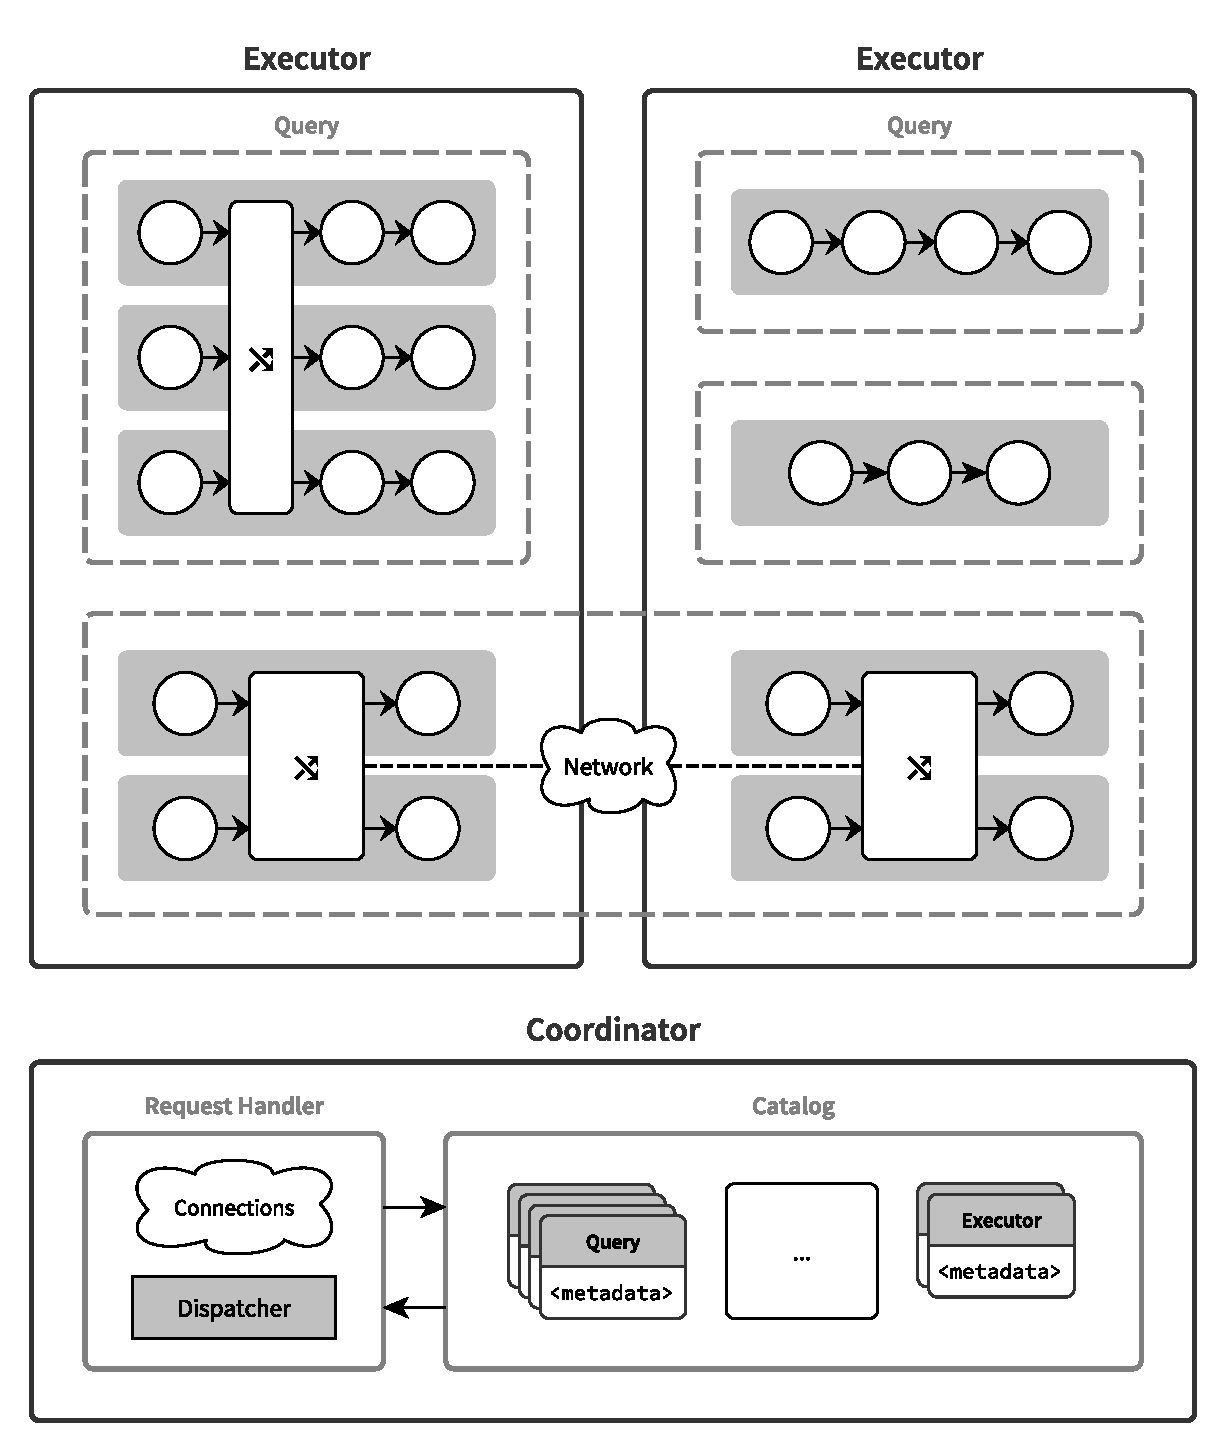
\includegraphics[width=1\textwidth]{figures/components}
  \caption[System architecture.]{ Queries (dashed boxes) consist of one or
  more worker threads (rounded grey boxes) driving the dataflow computation.
  A query might span over multiple executors, makeing use of the network for message exchanges
  between the workers of a query.\\
  The coordinator maintains a connection to every  executor and every query process.
  The state of the whole system is stored in the catalog.}
  \label{fig:components}
\end{figure}

\begin{table}
    \myfloatalign
  \begin{tabularx}{\textwidth}{>{\scshape}lX} \toprule
    \tableheadline{Component} & \tableheadline{Description} \\ \midrule
    Query & User-submitted Timely program running in the system.\\
    Worker & Thread belonging to a query, driving the computation of its local dataflow graph instance.  \\
    Executor & Process designated to host and spawn queries. \\
    Coordinator & Central process managing all the other components.\\
    Catalog & Data collection storing and exposing the system state at the coordinator.\\
    Topic & A named and typed representation of an exposed data stream.\\
    Publisher & Operator for exposing Timely streams by publishing them as a topic.\\
    Subscriber & Consumer of a stream emitted by a given topic.\\
    % submission
    % dataflow graph
    \bottomrule
  \end{tabularx}
  \caption{Terminology of the system.}  \label{tab:design-terminology}
\end{table}


\clearpage

\section{Queries}

A query is a Timely program managed and executed by our system. Like
standalone Timely Dataflow programs, queries are written in Rust and linked
against the Timely Dataflow library. The dataflow graph is constructed by connecting
Timely's operators (vertices) to stream objects (edges).

In standalone Timely applications, the user has to manually provide a configuration
for the worker threads. In our system, this information is partially generated by
the system, based on a user-provided template. Thus, we require that a query
registers its computational logic with our \lstinline{timely_query::execute} function,
instead of calling Time\-ly's initialization function directly.

This means that in order for a Timely Dataflow program to become a runnable
query in our the system, it needs to link against our \lstinline{timely_query} library.
This library not only performs the initialization of the Timely run-time, it also
provides additional functionality to interact with the coordinator, which we
describe below in section \fullref{sec:sharingstreams}.

Other than this, we do not want to impose any restrictions on what a query program
can do, it is free to execute arbitrary code.

\begin{lstlisting}[caption={[Example query.]Example query which prints out a stream of integers.}]
extern crate timely;
extern crate timely_query;

use timely::dataflow::Scope;
use timely::dataflow::operators::{Filter, Inspect, ToStream};

fn main() {
  timely_query::execute(|root, coordinator| {
    root.scoped::<u32, _, _>(|scope| {
      (0..100).to_stream(scope)
              .inspect(|x| println!("hello {:?}", x));
    });
  }).unwrap();
}
\end{lstlisting}

\section{Coordinator}

The coordinator is the central process of the system, managing all other
components. 
The coordinator provides an interface for users to submit new queries and
inspect the current state of the system. In order to receive commands and
report their internal state, every executor and query process maintains a
network connection to the coordinator.

Bookkeeping of the system is done by the coordinator in the catalog. The
catalog is a datastructure which contains all information about the available
executors, the running queries and their workers. This data is exposed to
queries through so called \emph{collection topics}, which we will describe
below. This allows queries to introspect the system state using Timely operators.

\subsection{Submission}

A query is submitted to the coordinator as a binary executable. Compilation
is done externally to allow the use of third-party libraries. A submission
consists of the location of the query binary, as well as the runtime
configuration for the workers. The runtime configuration specifies the amount
and distribution of the worker threads which will drive the query.

Optionally, a human-readable description of the query,
as well as the command-line arguments to be passed to the executable can be
provided.

When handling a new query submission request, the coordinator will assign a
unique identifier to the incoming query, and then select a
matching number of executors for the query to be spawned on. The selection
of executors is based on the runtime configuration provided by the submission
request.

The coordinator plays an important role when spawning new queries. After
issuing query spawn requests to the executors, it waits for all query processes
to register themselves at the coordinator before they begin their computation.
Only then the query is considered active and the submission request
is reported to be completed.

\begin{figure}[htb]
  \centering
    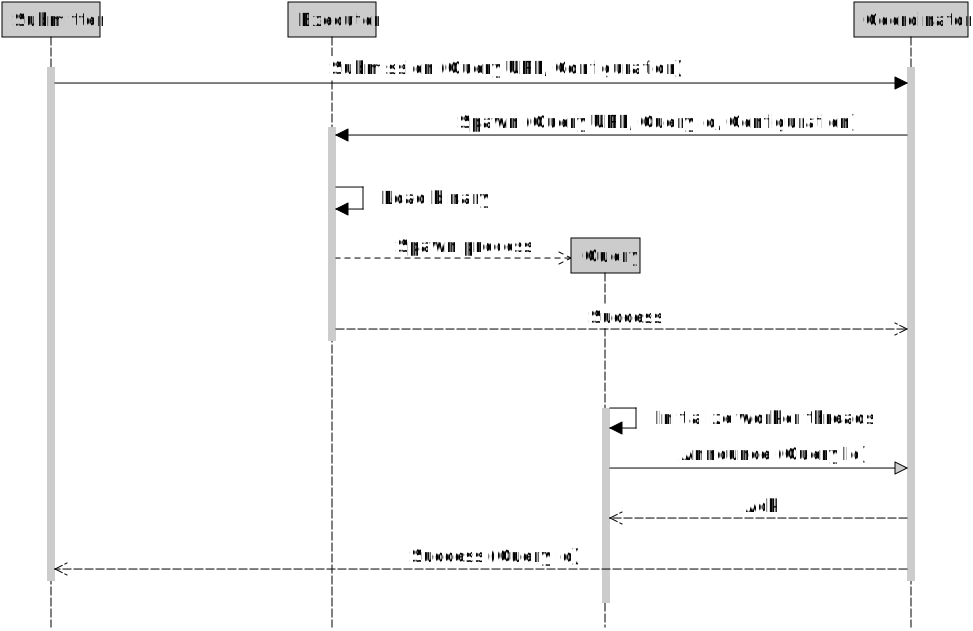
\includegraphics[width=1\textwidth]{figures/spawn_singleprocess}
  \caption[Query submission with single process.]{Submission of a query on a single executor.
  Only once the spawned query announces itself at the coordinator is it considered running.}
  \label{fig:subsingle}
\end{figure}

\section{Executors}

The spawning and direct supervision of query processes is not done by the
coordinator itself, but is offloaded to designated processes called executors.
This choice allows for more flexibility regarding query execution and the
management of available resources. Since executors can be dynamically added
to the system, and with some limitations also be removed again, they provide
a way for adding new machines to the cluster running our system. The catalog
maintains the pool of available executors which are participating in the system.

As a timely program can span over multiple machines, a query might span
over multiple executors. The placement of a query on the available executors
is performed by the coordinator, based on the users request.
We currently implement a naive approach to query placement, where the executors
are chosen randomly if the user does not manually specify a placement. A more
sophisticated scheduling, which for example could include load balancing,
has to be investigated.

Another feature of executors is that they define how queries and their
worker threads are supposed to be executed. When an executor joins
the system by introducing itself to the coordinator, the executor also informs
the coordinator about the execution format it supports. In the current
implementation, executors only support the execution of queries in the form of
native operating system executables.

When spawning such an executable, the newly spawned query process
performs the worker initialization on behalf of the executor. 
The executor supplies the newly created process with the information
it needs in order to participate in the system. This includes the query's own identifier,
the address of the coordinator, the addresses of any peer processes belonging to the 
same query, and the number of worker threads to spawn inside this process.

Executors are also responsible for fetching any query binaries they are supposed
to spawn. When submitting a new query, the submitter has to provide coordinator
with the location of the binary. This location is forwarded to participating executors,
which will use it to load the query binary. 

Since executors serve as a provider for computational resources such as machines,
there is typically a one-to-one mapping between executors and the machines they
are running on. This however is not a requirement of the system, the deployment of
executors is left to the user. Similarly, the user is free spawn multiple
processes belonging to the same query on the same executor if they wish to do so.

Since operating system processes can outlive their parent process, executors can
be removed from the system while the queries spawned by the executor are still
running. In this case, the coordinator removes the terminating executor from
the pool, disallowing any future queries to be hosted on the removed executor.

\paragraph{Future Considerations}

The current implementation of executors which run queries in their own separate
process is not the only possible implementation choice.
Alternative implementations could for example host multiple queries
within the same process, by dynamically loading the query's code into an already
running process and run it on a preemptive operating system thread. This would allow queries
the interchange of objects without the need for data serialization. Given
the implementation of Timely's operator scheduling, cooperative scheduling
of multiple worker threads within a single operating system thread could also
be implemented for certain queries where its input is managed by the system.


\section{Sharing Data Streams} \label{sec:sharingstreams}

Dataflow programs typically work on streams from external sources. As the same
data source might be of interest for different dataflow computations, it seems
appropriate to manage data streams in our system as well. Furthermore,
input streams might not only come from external sources: A dataflow computation
might produce an intermediate or final output stream which could be of interest
for other queries. These assumptions motivate us to extend our system with a
mechanism to allow queries to expose their data streams for consumption by other
queries.

We implement this in the form of a topic-based publish/subscribe system:
Using the \emph{publish} operator, a query can expose one of its streams
(an edge in the dataflow graph) to other queries, which in turn then \emph{subscribe}
to it. The list of all published topics is stored at in the catalog.

The reason for choosing a topic-based publish/subscribe system over a
content- or type-based one is dictated by the fact that Rust allows for little
type introspection. In addition, having users explicitly publish and name
exposed streams helps to differentiate between streams with the same datatype
but different semantics.

For providing access to external inputs, we require that a designated query
translates these external inputs into Timely streams and publishes the result as
a topic. We prefer this manual approach over providing our own adapters, as there
already exists a rich collection of Timely-aware code which performs this
translation of external input to Timely streams.

\subsection{Topics}

A topic has the following properties, which are all stored in the catalog
and can be accessed by other queries.
\begin{description}
\item [Identifier] A unique identifier for the topic instance.
\item [Name] When publishing a stream, the publisher has to assign a name to it.
Queries use this name to refer to topics they want to subscribe to. There might
be only one topic with a certain name at a time, however names can be reused if
topics are unpublished.
\item [Schema] A descriptor of the data type of the stream published in this
topic. Timely's streams are typed channels, therefore so are topics.
\item [Address] An address to which the subscribers connect in order to received
the contents of the published stream.
\end{description}

While every publication and subscription request is disclosed to the coordinator
and the catalog contains a list of all existing topics, the
actual exchange of data happens directly between queries. When a query subscribes
to a topic, it receives the address of the topic's publisher from the coordinator
and directly connects to it.

\subsection{Stream Publisher}

A stream publisher is a Timely operator which exposes a Timely stream as a topic. When
creating it, the query author has to assign a name for the topic under which the
input stream will be published. As with all other Timely operators, the publisher
operator is instantiated on all worker threads. However, the user can choose
whether all worker streams are merged into a single topic before publishing, or
if each worker publishes its own topic. The latter option implicitly exposes
the data sharding strategy of the publishing query, allowing the workers of
the subscribing query to exploit this partition scheme.

\subsubsection{Collection Publisher}

Our publishers are not buffered, meaning subscribers will
not receive any data which was produced before they subscribed to a certain
topic. This is the same as in many other publish/subscribe systems, where
synchronization between publishers and subscribers is decoupled as well. \cite{pubsub}

However, in streams where the contents of the stream describes changes of a certain
state, it is essential for stream consumers to know the state of the source at
the beginning of the stream in order to make sense out of it. The motivating
example here is the catalog, which is supposed to expose the current system state to
new participants.

For this reason, we introduce a second kind of publisher which publishes
\emph{collections} instead of streams. A collection in our model is a typed, unordered
multiset maintained by the publisher, possibly representing state it would
like to share with subscribers.

Upon creation, a collection publisher contains an empty collection.
When the publishing query mutates the collection by adding or removing elements,
these changes are propagated to the subscribers. When new subscribers connect
to this publisher, the publisher will provide them with a list of all currently
contained elements. This way, all subscribers eventually maintain the same view
of the data collection.

From the subscribers point of view, a topic published by a collection publisher
is not inherently different from a normal topic: After subscribing, it will
observe a continuous stream of data. The difference is in the data type of the
stream, it will be of tuples of the format $(\texttt{Data}, \delta)$, where
\texttt{Data} is an element that can be stored in the multiset and $\delta$ 
is a signed integer denoting the amount of elements that have been added or removed from the set.
This format is compatible with the notion of collections in Differential Dataflow \cite{differential},
allowing subscribing queries to further process the collection in a convenient
manner. Note however that our collections are not versioned, we
do not append timestamps to the update messages.

\subsection{Subscriber}

In order to subscribe to a topic, the subscribing query has to provide the name
of the topic it is interested in. This involves a name lookup which can optionally
be blocking: If a requested topic does not yet exist, the coordinator will add
the subscriber to a wait list. Once a corresponding topic is published under that
name, the coordinator will inform the subscriber about this topic. 

The subscribing query is free to subscribe to multiple topics. It the query's
responsibility to merge and feed the data streams into the dataflow graph.

\subsection{Comparison with Timely's Capture \& Replay}

The Timely library provides special capture and replay operators which also serve the
purpose of sharing data between queries. With the capture operator, all timestamp,
data and event records are collected in one dataflow computation,
and can then be replayed in another one.

The capture/replay operators will record and replay the whole stream from beginning
to end, requiring the capture operator to either buffer its incoming data or
wait for the replaying query to connect to it. 
In our system, we opted for a more dynamic approach, where
producing queries are allowed to discard data if there are no consumers.

It is the responsibility of the user to provide a communication channel between
capture and  replay operators. Adapters exist for Rust's thread-safe FIFO queues,
single-threaded queues, file handles and sockets.


\cleardoublepage
\chapter{Implementation}\label{ch:impl}

In this chapter, we discuss the implementation of the individual components
presented in the previous chapter, but we also present some shared implementation
features, such as the common request/response protocol used for the
communication between the different components.

\section{Coordinator}

As the central component of our system, the coordinator performs a rich
set of tasks. These involve handling submission requests to spawn new queries,
but also handling publication and subscription requests from existing queries.
It is the central authority about the current system state, i.e. it maintains
a list of all running queries and executors, but it also tracks all existing
publications and subscriptions. It exposes this information in the catalog.

Because most components interact with the coordinator, its
internal implementation is not without challenges. The two major ones
being the fact that it has to deal with many concurrent asynchronous events,
and secondly that it has to maintain shared mutable state.

Before we discuss these challenges, we provide a brief overview of the
internal architecture of the coordinator: To other components, the coordinator
exposes a request/response-based interface on a predefined networking port.
For this purpose, the coordinator listens for incoming connections on that port
and then waits for the connected clients to send requests. Once requests are
received and decoded, they are forwarded to a central request handler. This
request handler contains the central logic of the coordinator, keeps track of
unfulfilled requests and mutates the catalog to announce changes in the
system state.

\subsection{Dealing with asynchronous events}
The initial prototype of the coordinator used a multi-threaded approach for dealing
with multiple clients at the same time, and used message passing between threads
to avoid directly exposing shared state. However, many requests handled by
the coordinator require it to wait for external events, and thus a form of
cooperative task management is needed.

We initially used a continuation-passing style for splitting blocking requests into
non-blocking subtasks. However, due to Rust's memory ownership model, we found that
this approach often resulted in manual \emph{stack ripping} \cite{stackmgmt},
which made code both hard to read and inconvenient to write.

This motivated us to re-design the coordinator around a central event loop, which
allows us to multiplex many asynchronous tasks within the same thread. However,
instead of using raw callbacks as event handlers, we decided to adapt an external
library called \lstinline{future-rs} \cite{futuresrs}. It provides a more expressive interface
for dealing with asynchronous tasks based on the concept of \emph{futures}. Futures
(sometimes called promises, eventuals or deferred objects) are proxy objects for
values that will eventually be provided through some asynchronous event.
The \lstinline{future-rs} library provides combinators for chaining events
together or waiting on multiple events at the same time. Actions on completed
futures are expressed as closures. This means that stack ripping occasionally still
occurs, however the fact that the completion handlers are chained together
allows for a more sequentially looking code.

A unique aspect of the implementation of \lstinline{future-rs} is that futures
need be polled in order to make progress. When a future is polled, it checks
if any pending events have occurred and if so, dispatch any pending completion
handlers. It is the users responsibility to ensure that futures are being
polled. This is typically done by registering the future in an event loop.

\subsubsection{Event Loop}
The \lstinline{future-rs} library itself provides a set of primitives to
create and combine futures, it also provides abstractions for expressing which
events a future is waiting for, and expressing the occurrence of events, it
does however not provide an implementation of an event loop. Our implementation
of the coordinator thus provides a simple event loop whose sole task it is
to wait for events to occur and poll registered futures accordingly.

To avoid having to pass around a handle to the event loop, it stores its 
list of waiting futures in thread local storage. The public interface consists 
of two free-standing functions, \lstinline{async::spawn} for registering
new futures to the event loop, and \lstinline{async::finish} for initializing
the event loop and waiting for its termination. \lstinline{async::finish} accepts
also initial the initial future which is used to register further futures in
the event loop. The motivation for this interface, which arguably looks
a bit uncommon for an event loop, stems from the fact that we model each
concurrently running task as a chain of futures, basically treating them as
coroutines.  

Listing~\ref{lst:coorddispatch} shows an example of this. Our networking layer
models the server socket as a future which yields a stream of incoming connections.
Each connection itself then maintains a queue for incoming requests, which is
also modeled as a future, allowing the user to specify actions to be taken
once a request is received.

\begin{lstlisting}[caption={[Connection handling at the coordinator]%
Accepting and dispatching incoming connections. The actions specified
in \lstinline{for_each} and \lstinline{map_err} are invoked by the
event loop if the corresponding events (such as new incoming connections,
new incoming requests or errors during request handling) occur.},label={lst:coorddispatch}]
// `listener` is future yielding a stream of accepted connections
let listener = network.listen(9189);
// define the action to be executed for each incoming connection
let server = listener.for_each(|connection| {
    // queue pair for outgoing/incoming requests
    let (tx, rx) = connection;
   
    // this action is invoked for each incoming request
    let client = rx.for_each(move |request| {
        // decode and dispatch request 
        ...
    }).map_err(|err| {
        // futures can also yield error values
        // which are handeled separately
        error!("failed to dispatch request: {:?}", err)
    });

    // register client handlers in event loop
    Ok(async::spawn(client));
});

// drive the event loop to completion
async::finish(server);
\end{lstlisting}




With this abstraction, requests that might be completed asynchronously
%(i.e. a blocking subscription request for a topic which has not yet been registered)
are split up into a future representing the pending response, and a completion handle
which is invoked once the request can be resolved. Bookkeeping of pending requests
is done in the request handler.



\subsection{Maintaining shared mutable state}

The nature of the coordinator requires it to mutate its internal state on
behalf of the connected clients. As the Rust programming language discourages
the use of aliased directly mutable references, we have to provide a wrapper
type which allows the connection handlers mutable access to the request handler.

Because all requests originating from a certain connection are issued using a
wrapper, we can use it to keep track of the requests submitted by that connection.
This allows us to clean up any associated state if the connection disappears,
such as removing disconnected executors from the pool, or depublishing 
topics of crashed workers.

\subsection{Catalog}

The purpose of the catalog is to maintain and expose the current state of the
system. It tracks the addition or removal of executors, queries, topics,
publication and subscriptions and exposes them in collection topics according
to the schema shown in Figure~\ref{fig:model}.

\begin{figure}[htb]
  \centering
    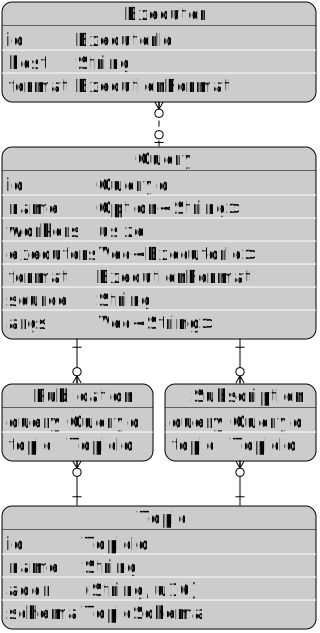
\includegraphics[width=0.5\textwidth]{figures/model}
  \caption[Schema of the catalog.]{Schema of the catalog. All five data types
  are published as a collection topic, allowing users to follow state changes
  in the system.}
  \label{fig:model}
\end{figure}

The catalog itself only exposes this data. It is mutated and queried by the
request handler in order fulfill certain requests.

\section{Executor}

The current implementation of the executor is relatively simple. It is an executable
that registers itself at the coordinator and then spawns child processes on behalf
of the coordinator.

In order to add a new host to the cluster, the user has to deploy the executor
binary on the new host, specify the address of the coordinator and then launch
the executor binary. The executor registers itself at the coordinator, which
assigns a unique identifier to the connecting executor. Once connected to the
coordinator, the executor listens for incoming spawn requests. If such a
request arrives, it fetches the binary from the specified source and launches
it as an operating system process. Any command line arguments to be passed
to the query are provided here as well.

The executor has to inform the spawned binary about its assigned query identify,
the address of the coordinator and the address of any peer processes. In the
current implementation this is simply done using environment variables, which
can easily be accessed by the spawned query.

% TODO talk about supported url formats
% TODO talk about stdout forwarding

\section{Query Library}

We provide a small wrapper library which allows Timely processes to participate
in our system. A query submitted to the system must eventually call the 
\lstinline{timely_query::execute} function, a function which mirrors Timely's
own \lstinline{execute} function. When called, this function parses the
environment variables mentioned above which are provided by the executor.
Using this information, the process connects to the coordinator and registers
itself by providing its identifer and the group of workers it will host. Once
all worker groups have successfully registered themselves at the coordinator,
the coordinator replies with a randomized token which is used to identify
the registered processes belonging to a query. 

The initialization of the Timely worker threads and the allocation of the
communication channels among them is done using \lstinline{time\-ly_\-com\-mu\-ni\-ca\-tion}
the same way as it would be done in a standalone Timely program. For this
reason, our query library needs to translate the information provided by the
executor into Timely's own format.

Our query library also needs to provide an interface for worker threads to
publish or subscribe to topics. For this reason, every worker thread gets
a handle for the connection to the coordinator. Access to the
publish \& subscribe system is provided through a set of remote
procedure call stubs which are described in the following section.

\subsection{Publishers \& Subscribers}

The query library exposes the publish and subscribe functionality. The following
API is used for publishing and subscribing to Timely streams.

\begin{lstlisting}[caption={[Publish \& subscribe interface]
The interface for publishing and subscribing Timely streams.
}]
pub struct Coordinator {
  /* hidden handle to request queue */
}

impl Coordinator {
  pub fn publish<S, D>(&self, name: &str, stream: &Stream<S, D>,
    partition: Partition) -> Result<Stream<S, D>, PublicationError>
      where D: Data + NonStatic, 
            S: Scope,
            S::Timestamp: NonStatic;

  pub fn subscribe<T, D>(&self, name: &str, cap: Capability<T>) 
    -> Result<TimelySubscription<T, D>, SubscriptionError>
      where T: Timestamp + NonStatic, 
            D: Data + NonStatic;
}
\end{lstlisting}

The \lstinline{NonStatic} bounds on the data and timestamp
parameters are required for safe serialization described in \ref{sec:serialization}.

\subsubsection{Publisher}

The \lstinline{publish} function takes a direct reference to a Timely
\lstinline{Stream<S, D>}. These stream handles, which are only available during
the dataflow graph construction phase, allow us to instantiate our own publish
operator on the stream.  The instantiated publish operator will push both, its
incoming data, as well as its current frontier to any subscribers. 

Once the operator is inserted into the dataflow graph, the \lstinline{publish}
stub issues a registration request to the coordinator, which will result in the
creation of a topic for other queries to subscribe to.

The \lstinline{partition} argument on the API specifies whether all streams
shall be merged into a single topic, of if every worker publishes its own stream.
In the second case, the identifier of the publishing worker is appended to the
name of the topic:

\begin{lstlisting}[caption={
Example use of publisher.
}]
timely_query::execute(|root, coord| {
    root.scoped::<u64, _, _>(|scope| {
        let i = scope.index();
        let numbers = (i*100..(i+1)*100).to_stream(scope);

        // results in `n` topics:
        //    "numbers.0", "numbers.1", .., "numbers.n"
        coord.publish("numbers", &numbers, Partition::PerWorker)
             .expect("failed to publish topic");

        // filtering performed by each worker in parallel
        let primes = numbers.filter(|x| x.is_prime());

        // results in a single merged topic called "primes",
        // published by worker number 0
        coord.publish("primes", &primes, Partition::Merge)
             .expect("failed to publish topic");
    });
})
\end{lstlisting}


\paragraph{Collection Publisher}

In addition to the stream publisher, we also provide the so called collection
publisher. It has a similar interface for publishing, but it requires the
type of the incoming stream to deliver \lstinline{(D, i32)} tuples, where
the integer denotes the amount of elements have been added or removed from
the collection.

\begin{lstlisting}[caption={[Collection publisher interface]
}]
impl Coordinator {
  pub fn publish_collection<S, D>(&self, name: &str,
    stream: &Stream<S, (D, i32)>, partition: Partition)
    -> Result<Stream<S, (D, i32)>, PublicationError>
      where D: Data + NonStatic, 
            S: Scope,
            S::Timestamp: NonStatic;
}
\end{lstlisting}

Internally, the publisher maintains a copy of this collection. This is required
for new subscribers, which must be informed about the contents of the collection
when they connect.

Both publishers share the same underlying logic which accepts incoming connections
from subscribers and provides notifications for disconnected clients.



\paragraph{Implementation Details}


Internally, this logic also make use of the \lstinline{future-rs} library, 
since futures have also been integrated in our networking layer. A unique
aspect of the futures provided by \lstinline{future-rs} is that they need
be polled in order to make progress.

Inside the coordinator the polling is done by its event loop. For the futures
inside our publish and subscribe operators however we make use of the fact
that Timely itself also uses polling-based scheduling. This guarantees that
the surrounding Timely operator is polled regularly, enabling it to poll
the contained futures for completion.

\subsubsection{Subscriber}

In contrast to the publisher, the current implementation of the \lstinline{subscribe}
function does not directly instantiate a Timely operator, but returns a subscription
handle which is used to read data from the topic.

There are two reasons for this choice: First, Timely requires that an operator
is instantiated on every worker. It can happen that the amount of topics a query
would like to subscribe to and the amount of workers do not match. Thus, the API
quickly becomes complicated, as we would need to provide an interface assigning
topics to operators.
Second, Timely's operator contract requires that an operator instance announces
the internal initial capabilities it holds, and, more importantly, the initial
capabilities of its peers. To support this would require some synchronization
between the subscribers, as they have to exchange the initial frontier they
observe at their topic.

Instead, we decided to base our subscription progress tracking on Timely's new
capability handles. The recently added \emph{unordered input operator} allows
a query to feed a computation from data with unordered timestamps. This operator
exposes a root capability for the earliest possible timestamp, allowing the user
to derive capabilities for newer timestamps from old ones. The frontier
is advanced by dropping the capabilities for timestamps for which no more data
is pending.

Based on the progress tracking information delivered by the publisher, the
subscription handle will automatically derive new capabilities for incoming
data and drop old ones if the frontier advances. The user however has to
provide the initial root capability for the input.

\begin{lstlisting}[caption={[Typical use of the subscription handle]
Typical use of the subscription handle. This query subscribes to a single topic of
strings, with \lstinline{u64} being the type of the timestamps.
}]
timely_query::execute(|root, coord| {

    let (mut input, cap) = root.scoped::<u64, _, _>(|scope| {
        let ((input, cap), stream) = scope.new_unordered_input();
        // stream.operators(..)
        (input, cap)
    });

    let topic = coord.subscribe::<_, String>("example", cap)
                     .expect("failed to subscribe");

    for (time, data) in topic {
        let session = input.session(time);
        session.give_content(&mut Content::Typed(data));
        root.step();
    }
})
\end{lstlisting}

In queries which use multiple workers, the query author can decide which workers
actually subscribe to topics, as the code outside the graph generation is allowed
to conditionally decide if it wants to call the subscribe function. Because
the root capability can be cloned, this interface also allows the user to
interleave the data from a topic with other data, for example by merging
multiple topics at the input.

\section{Shared Communications Layer}

For the remainder of this chapter we discuss the networking and communications
layer of our system, which is used all components for implementing their
services.

\subsection{Messaging}

Our system consists of potentially many distributed processes. These processes
are running concurrently, are dynamically added and removed from the system
and are communicating with each other. In order to deal with the inherent
complexity of such a system, we adopted an actor-model like approach for our
implementation.

Actors in our system include processes like the coordinator, the executors 
and the query processes. However, as Timely by itself could be seen as an
actor system, operators like the publish or subscribe operators are also actors
directly interacting with our system.

To support this kind of model, our networking layer also works in terms of
asynchronous messages. In contrast to Timely's own networking layer which also
provides a similar abstraction, we cannot assume a fixed number of actors.
In order to establish a connection between two components, one of them has to
take on the role of the server, while the other one acts as a client. Two
queues are allocated per connection on each actor: one for incoming messages
and one for outgoing messages. This enables messages to be sent asynchronously
in both directions. Network failures are signaled in the queue for incoming
messages. Currently, Rust's standard library TCP sockets are used as the
underlying transport mechanism, however the system could easily be extended to
support alternative transport layers as well.

\subsection{Request \& Response Messages} \label{sec:reqresp}

While the abstraction of single messages is sufficient for implementing the
mostly unidirectional messaging paradigm of the publish-subscribe implementation,
most other communication in the system follows a request-response pattern.
For this reason, we implemented a request-response multiplexer on
top of the plain message channels. This multiplexer allows both actors to have
multiple requests in flight while waiting for the corresponding responses,
which can be delivered out of order.

In order to differentiate between different kind of requests and also ensure a
well-typed response format, request payloads have to implement the \lstinline{Request}
trait. The associated name is used for decoding, while the associated \lstinline{Success}
and \lstinline{Error} types specify what kind of payloads are valid for the response.
This allows the response for a given request \lstinline{R} to be represented by
Rust's \lstinline{Result<R::Success, R::Error>} type.

\begin{lstlisting}[caption={[Request trait]In order for a type to be used as a
request message, it needs to implement the \lstinline{Request} trait. The name allows
request handlers to differentiate between different types of requests, while the associated
types forces them to issue well-formed responses.
The trait bounds are explained in section \ref{sec:serialization}.}]
pub trait Request: Abomonation + Any + Clone + NonStatic {
    type Success: Abomonation + Any + Clone + NonStatic;
    type Error: Abomonation + Any + Clone + NonStatic;

    fn name() -> &'static str;
}
\end{lstlisting}

\subsection{Serialization} \label{sec:serialization}

For both, the request/response messages as well as messages used in the publish/subscribe
subsystem, we need to serialize the payloads in order to send them over the network.

\subsubsection{Message Buffers}

Incoming and outgoing network data is stored in reference counted message buffers.
This buffer supports multi-part messages, meaning a message contains more than
one serialized object. This is needed for the request/response multiplexer, which
needs to partially decode a message in order to determine to which request it
belongs to. It is also used in the publisher and subscribers, which allows them
to encode and decode the timestamp and the data separately.

Reference counting is an optimization used by publishers, which allows them to
serialize the data only once and share the buffer with all subscribers. Every
outgoing queue to the subscriber only contains a reference to the buffer. Once
the message is written to the subscriber's socket, the reference count is
decreased and the message is deallocated once all subscribers have consumed it.

\subsubsection{Safe Serialization with Abomonation}

Timely itself provides a uses a high-performance serialization library called
Abomonation, implying that all data types sent to a publish operator will be
serializable this way. This makes Abomonation a natural choice as the serialization
format for the messages sent from publishers to subscribers. 

However, Abomonation is neither memory- nor type-safe. There are no safeguards
against deserializing data into an incompatible type, which will result in undefined
behavior. In Timely, such errors are typically avoided since all worker
execute the exact same program code and the streams between workers are
statically typed. In our system however, a publisher might accidentally use
a different version of a library type than the subscriber. Because of this,
we use our own lightweight wrapper around Abomonation. In addition to the raw
serialized bytes, we annotate the buffer with the \lstinline{TypeId} of the
data type. Rust's \lstinline{TypeId} provides an opaque, globally unique
identifier for a given Rust type and its representation. Thus, we can check
if the expected and provided type identifier match before trying to deserialize
a message.

In order for a type to be serialized by our library, it needs to fulfill the
following type bounds: \lstinline{Abomonation + Any + Clone + NonStatic}.

The \lstinline{Any} trait is required to retrieve the type's identifier. The
\lstinline{Clone} trait is used to put deserialized types into the incoming
messages queue and \lstinline{NonStatic} is an auto-trait used to disallow the
creation of eternally valid pointers into temporary buffers. We also take type
alignment rules into consideration when serializing into unaligned buffers. 

\paragraph{Alternative Serialization Formats}

We currently use our safe Abomonation wrapper not only for data in
publish/subscribe system, but also for serializing and deserializing requests
and response messages. This implies that currently all participating components
have to be compiled for the same processor architecture and operating system.

Because of this, our message buffer interface has been designed to use alternative
serialization formats in the future. Besides supporting heterogeneous clusters,
alternative formats might also be useful in the publish/subscribe system:
Schema-based serialization formats would allow subscribers to decode published
data even without static knowledge of its data type.

\begin{comment}
\section{Dealing with asynchronous requests} \label{sec:futures}

Our components are dealing with many concurrent events from different sources
at the same time. When spawning a new query for example, the coordinator not
only has to wait for acknowledgments from the executors, it also has to be
ready to deal with the incoming connections from the newly spawned queries. And
ideally, we would like the system to be able to continue processing requests
while it waits for responses from other components.

The initial prototype of the coordinator used a continuation-passing style
for requests which could not be completed immediately. However, due to
Rust's memory ownership model, we found that this approach often resulted
in manual \emph{stack ripping} \cite{stackmgmt}, which made code both
hard to read and cumbersome to write. This lead us to consider the use of an
external library to deal with this kind of asynchronous task management.

One possible solution such library we considered is Timely Dataflow itself, which could
be used to model the coordinator as a dataflow computation.
While we think that this is certainly possible, we found the fact that Timely
has a static dataflow graph would would have required us add an additional
multiplexing layer at the inputs and outputs, complicating the code. 

In addition, Timely currently requires all data to be serializable. Because
the coordinator deals with non-serializable resources such as socket handles,
we would still require a solution to deal with asynchronous events when dealing
with I/O.

The current implementation uses the \emph{futures-rs} library for modeling
asynchronous tasks. It provides abstractions for both asynchronous computations
that yield a single result, a \lstinline{Future}, and computations that
continuously produce results which implement the \lstinline{Stream} interface
(not to be confused with Timey's stream handles). The library provides combinators
for the user to chain these asynchronous requests together or register actions
to be taken once the asynchronous request is completed.

The \emph{futures-rs} library itself however does not provide an event loop
which reacts on events and resolves pending futures. For this reason, we implemented
our own event loop. \TODO{This is crap}

A notable difference between \emph{futures-rs} and other future-based libraries
is that it is polling based, which fits well with Timely's execution strategy
for operators, which are also polled.

\end{comment}

\cleardoublepage
\chapter{Evaluation}\label{ch:evaluation}

For our experimental evaluation we split a monolithic dataflow computation into a
modular set of queries. The modular queries share their results in a topic,
allowing subscribers to further process the data. Because queries
can be dynamically added to the system, there is no need to interrupt the
running computation if additional analysis stages have to be added.

This increased flexibility comes however at a cost. As data has to be published
in topics in order to be accessed by consuming queries, we expect there to be
some overhead in both memory consumption and processing latency. The goal
of this chapter is to measure and analyze the overhead of query composition
on a realistic workload.

\paragraph{Experimental setup}

All experiments are executed on a dual-socket Intel Xeon E5-2650
machine (2.0GHz, 8 cores per socket, 2 threads per core) with 64 GB RAM. All components and
queries in our system are compiled with a Rust 1.14 nightly build (2016-10-20)
and executed on Debian 7.8. The input data is read from a SAN storage attached
via iSCSI on a private 10 Gbit Ethernet network.

\section{Query composition for sessionization}

The dataflow computation in this experiment is based on \emph{sessionization},
i.e. the reconstruction of user sessions from a trace of log events.

\subsection{Computation \& workload}

The workload in this experiment is an hour-long trace of log events, collected in
a large datacenter owned by an provider for the travel industry. The messages in our trace were
accumulated concurrently by 42 log servers, which received their log events from
1263 different streams. Events are originating from a distributed middleware which acts
as a message broker. It records metadata about the received messages, such as
timestamp, session identifer, and transaction identifer, and forwards them to
the log sever.

The computation we use on this workload is called \emph{sessionization}. Sessionization
is the reconstruction of user sessions, i.e. grouping and then processing all
messages belonging to the same session. For this purpose, the computation waits for
the arrival of late messages before it can consider the session closed. In
our experiment we use a fixed inactivity limit of 5 seconds, and re-order messages
within an event time window of 10 seconds. This is enough to incooperate more
than 99.99\% of all messages. 

While sessionization has been designed for real-time processing on a live
stream of events, we will load the workload trace from disk for our experiments.
This not only simplifies the experimental design and ensures reproducibility,
it also allows us to explore the behavior of the system if there are only a
few worker threads.

\subsection{Dataflow graph}

Input is read from disk and fed into the dataflow graph in parallel, each worker
is responsible for a partition of the log servers. The read messages are sent
into the sessionization stage, where all messages belonging to the same session
are grouped together.

After the sessionization, the computation performs a set of statistics on the
reconstructed sessions. The stages are described below, the resulting dataflow
graph is shown in Figure~\ref{fig:monolith}

Messages are shuffeled according to their session identifier for the
sessionization stage, and are processed in parallel until statistics are
collected for the output, which is emitted at a single worker. 

\begin{description}
\item [Input] Parses the input files and feeds them into the sessionization stage.
\item [Sessionization] Distributes and then groups messages according to their session identifier.
Emits groups of messages belonging to the same session after a period of inactivity.
\item [Messages per Session] Simply counts and emits the number of messages belonging to a session.
\item [Duration of Session] Calculates the timespan between the first and last message of a session.
\item [Parse Transaction Trees] Parses the transaction identifiers for tree extraction.
\item [Transaction Tree Depth] Calculates the depth of the transaction trees.
\item [Top k Transaction Tree Signatures] Calculates signatures for the transaction trees and
reports the ten top most common tree signatures.
\item [Top k Communication Pairs] Infers the ten most common pairs of services who are
communicating with each other.
\item [Output] Collects emitted data in a histogram.
\end{description}

\begin{figure}[p]
  \centering
    \includegraphics[width=1\textwidth]{figures/sessionize_dataflow-crop}
  \caption[Dataflow graph for monolithic sessionization]{The dataflow graph
  for the original, monolithic sessionization query.}
  \label{fig:monolith}
\end{figure}

\begin{figure}[p]
  \centering
    \includegraphics[width=1\textwidth]{figures/sessionize_split-crop}
  \caption[Dataflow graph for modular sessionization]{Structure of the modular
  sessionization. Two topics are introduced connect the tree of queries.}
  \label{fig:split}
\end{figure}

\subsubsection{Splitting up the dataflow graph}

For this evaluation we split up the computation such that each stage represents
its own sub-query. In order to achieve this, we introduce two topics: The topic
\emph{sessionize} contains the result of the sessionization stage, i.e. 
the groups of messages belonging to a session. The second topic, named
\emph{transactions}, is introduced for the transaction-oriented statistics.
It emits a stream containing all the transactions per session. The resulting
modular dataflow graph is shown in Figure~\ref{fig:split}, it consists of
seven queries, each one running in its own operating system process.


\paragraph{Topic Partitioning}

We maintain a simple one-to-one mapping between the number of topics and
number of worker threads in both the publishers and the subscribers.
Merging the stream partitions for publication and redistributing
the data at each subscriber would just result in unnecessary work.

\subsection{Worker-to-processor mapping}

We use the same amount of workers for each query to simplify topic partitioning.
But because the modular version naturally consists of more than one query,
the execution of the modular version will spawn more operating system threads
than the monolithic version.

For this reason we limit the the available CPU cores for the different executions,
ensuring the number of workers per query matches the number of available CPU cores.
Because our machine does have two processor sockets, each with their own memory bank,
the question arises how performance is impacted by different processor placement
policies. We explore this in section~\ref{sec:evalnuma}.

If not stated otherwise, we prefer using as many physical cores 
as possible before falling back to hyper-threads, and we prefer filling the
first socket before allocating threads on the second socket. The memory
allocation policy is set up to always allocate on the local node.

Note that we do not pin individual worker threads to individual cores, we just
disallow access to excess cores. The operating system is free to load-balance
threads between the available cores.

\clearpage

\section{Results}

\subsection{Overhead in execution time}

We report the overall execution time of of both the monolithic and the 
modular query for different amounts of worker threads in Figure~\ref{fig:times}.

\begin{figure}[htb]
  \centering
    \includegraphics[width=1\textwidth]{figures/evaluation/times}

    {\footnotesize
    \vspace{1em}
    \begin{tabularx}{\textwidth}{ rXXXXXX }
      \hline 
      \textsc{Threads} & 4 & 8 & 12 & 16 & 24 & 32 \\
      \hline 
      \textsc{Overhead} & 17.2\%&13.7\%&14.0\%&18.8\%&14.4\%&13.5\% \\
      \hline
    \end{tabularx}
    }
    \caption[Execution times for different number of workers]{
    Execution times for different number of workers, for both the monolithic
    and the modular version.}
    \label{fig:times}
\end{figure}

As expected, we see that the modular version is slower than its monolithic
counterpart. Where the monolithic query uses in-memory queues to send data
to the next stage, the participants of modular version have to serialize
the messages and publish them in a topic. Both versions do not necessarily
perform better if we use hyper-threading for additional worker threads,
as 24 workers in both cases perform worse than 16.

Previous work has shown that sessionization is able perform real-time processing
on this machine with 16 workers and more. Our monolithic version is indeed also
able to finish the computation in under one hour with 16 workers and more.
The modular version however only achieves execution times below the threshold
of one hour with 32 workers. Further work has to be done to investigate where
exactly the overhead comes from and optimize our system accordingly, such that
we achieve real-time performance with less workers.

The relative overhead varies between 13-18\%. It should be noted that relative
overhead is not proportional to the number of worker threads. We will show
in section~\ref{sec:evalnuma} that other factors such as placement also
impact the overhead.

\subsection{Worker utilization factor}

In this section we present the average measured utilization \emph{per worker},
i.e. the proportion of time a worker thread performs useful work.
This gives us an indicator of how well the different queries of the modular
version are able to cope with the given load.

We define the utilization factor of a worker as the percentage of
the time spent inside the Timely computation, i.e.
$\text{utilization} = \frac{\text{busy time}}{\text{total time}}$.
To put it another way, a worker is \emph{not busy} if it is waiting on external input.
This is the case if it wait on input from a topic in the case of the subscribers, 
or if it reads data from disk in the case of the sessionization stage.

Figure~\ref{fig:subutil} shows the average utilization for the subscribers, while
Figure~\ref{fig:sessutil} shows the utilization for the whole monolithic query
compared to the sessionization stage of the modular query. 

We see that in all cases the average utilization in the sessionization workers
is significantly higher than in the other queries of the modular version. This indicates
that the sessionization stage itself the bottleneck of the computation. 
We see that with a high number of worker threads, individual workers are proportionally
spending more and more time waiting for input.

This suggests that using the same amount of workers for all queries might
not be the most efficient use of computational resources. Future experiments would have to
explore how many worker threads are actually necessary for the different queries
in order to keep up. This however also requires a more sophisticated assignment of
topics to subscribing workers, which currently has to be manually encoded in
the queries source code.

\begin{figure}[p]
  \centering
    \includegraphics[width=1\textwidth]{figures/evaluation/subsutil}
    \caption[Subscriber worker utilization]{Utilization for the individual
    subscribers in the modular version.}
    \label{fig:subutil}
\end{figure}

\begin{figure}[p]
  \centering
    \includegraphics[width=1\textwidth]{figures/evaluation/sessutil}
    \caption[Sessionization worker utilization]{Utilization of the sessionization stage
    in the monolithic and the modular version.}
    \label{fig:sessutil}
\end{figure}
\clearpage
\subsection{Memory consumption and processor utilization}

Figures \ref{fig:rss} and \ref{fig:cpu} report the processor utilization and peak
memory consumption for the different processes, as reported by the operating
system.

\paragraph{Memory consumption}

We immediately see that the sessionization query of the composed version
consumes the most memory. This is caused by the fact that the re-ordering
and sessionization buffers incoming messages until certain epochs are completed.
Also with regard to the sessionization query, we see that its memory footprint
is higher than memory consumption for the monolithic version, even though
it performs less work. We assume that this is caused by the queuing of
outgoing messages at the publisher.

Another contributing factor to the overhead is the fact the we run additional
operating system processes, each one with a large set of worker threads.

\TODO{maybe split the figure in two separate figures, one for the subscribers
and one for sessionization}

\paragraph{Processor utilization}

We also report the overall processor utilization reported by the operating system.
A value of 100\% would correspond to the full utilization of all 32 logical cores.
We see that neither versions manage to fully utilize the processors over then duration of
the whole computation. This is indicates that both versions are sometimes blocked
on external input. Consistent with the observations from worker utilization, we
also see that the sessionization stage is the most compute heavy.

\begin{figure}[p]
  \centering
    \includegraphics[width=1\textwidth]{figures/evaluation/rss}

    {\footnotesize
    \vspace{1em}
    \begin{tabularx}{\textwidth}{ rXXXXXX }
      \hline 
      \textsc{Threads} & 4 & 8 & 12 & 16 & 24 & 32 \\
      \hline 
      \textsc{Overhead} & 7.9\%&10.3\%&10.6\%&9.7\%&13.7\%&13.5\%\\
      \hline
    \end{tabularx}
    }
    \caption[Peak memory consumption]{Peak memory consumption of the different
    processes. The left bar shows the monolithic query, the right bar shows the memory
    used per query processed of the composed version.}
    \label{fig:rss}
\end{figure}

\begin{figure}[p]
  \centering
    \includegraphics[width=1\textwidth]{figures/evaluation/cpu_tot}
    \caption[Total CPU utilization]{CPU utilization for the different
    processes. The left bar shows the monolithic query, the right bar shows the
    processor utilization for the different query processes in the modular version.}
    \label{fig:cpu}
\end{figure}
\clearpage
\subsection{Impact of worker placement} \label{sec:evalnuma}

In the above experiments, we prefer running as many workers as possible
on a single processor socket (with the exception of hyper-threads).
Figure~\ref{fig:numa} compares execution time of this strategy compared to a
strategy where we balance the workers evenly between sockets. With 12 workers
we are unable put all threads on a single socket, and we see that in this case
it is slightly beneficial to balance the threads evenly.

The impact of using different placements is relatively small for the
monolithic query. The modular version however is more sensitive to
different placement strategies, resulting in changes to the overhead
of the execution time. 

\begin{figure}[h]
  \centering
    \includegraphics[width=1\textwidth]{figures/evaluation/numa}

    {\footnotesize
    \vspace{1em}
    \begin{tabularx}{\textwidth}{ r|XX|XX|XX }
      \hline 
      \textsc{Threads} & \multicolumn{2}{c|}{4} & \multicolumn{2}{c|}{8} & \multicolumn{2}{c}{12} \\
      \hline 
      \textsc{Placement} & (2, 2)&(4, 0)&(4, 4)&(8, 0)&(6, 6)&(8, 4)\\
      \hline 
      \textsc{Overhead} & 22.9\%&17.2\%&17.9\%&13.7\%&17.3\%&14.0\% \\
      \hline
    \end{tabularx}
    }
    \caption[Execution time for different of worker placement]{Execution times for
    different worker-to-processor mappings. The placement describes the number of
    worker threads placed on each of the two processor sockets.}
    \label{fig:numa}
\end{figure}

\clearpage
\section{Discussion}

In this chapter we presented an experimental evaluation of the overhead of
query composition in our system. The results show that the modular version in
our setting takes about 13-18\% longer to execute and consumes 8-14\% more
memory. While this is not negligible, we are confident that a modular version
of sessionization would be able to keep up with real-time processing, given
enough resources.

We believe though that further experiments are indispensable to definitely 
answer this question. Unfortunately we were not able to conduct more experiments
within the remaining time.

For one, future experiments should evaluate the performance of modular sessionization
in a cluster of machines. We only ran our experiments on a single machine, meaning that
data shared in topics was transmitted over the loopback interface.
Having publishers on one machine and subscribers on another would certainly yield
different performance characteristics. The monolithic version would also
likely show a different performance behavior, as workers would have to shuffle their data over the
network instead of using shared memory queues.

In addition, we did not perform any microbenchmarks to evaluate the performance
characteristics of other features of our system, such as the latency
of spawning a new query or the time it takes to subscribe to a topic. While
this would be interesting to evaluate, it currently would only be of little
significance for long-lived queries such as sessionization, as we expect
these features mostly to be used during the set-up phase of a query.

\cleardoublepage
\chapter{Discussion}\label{ch:discussion}

\section{Related Work}

\subsection{Dataflow and streaming engines}

In contrast to the standalone Timely Dataflow library, many state of the art
dataflow streaming engines have been designed and engineered from the start
to run multiple current dataflow computations in a cluster. Thus, in this
section, we will mainly focus on the execution and management aspect running
multiple dataflow computations, and not so much on the programming model these
other systems provide.

It should be noted that in contrast to Timely and our system, all of the
following systems implement some form of fault tolerance. 

\subsubsection{Spark Streaming}

Spark Streaming \cite{sparkstreaming} is a streaming engine based on the Spark
cluster computation framework. Spark Streaming executes streaming dataflow
computations by turning them into stateless, fault-tolerant batch computations.
These batches are submitted as tasks to the underlying Spark engine. \cite{spark} 

\paragraph{Process Model}

In Spark, computational tasks work are modeled as transformations on partitioned
collections of records called \emph{resilient distribute datasets}. The
runtime schedules the execution of the transformations on a distributed set of
worker nodes. By tracking the lineage of transformations, Spark is able to
recover computations by reissuing lost transformations. Based on the model,
Spark Streaming models stateful, conceptually continuous dataflow computations
as small stateless microbatches.

This model of execution is very different from Timely's continuous operator
model. In Timely, both the operator scheduling and the data of the
computation are managed directly by the workers themselves, which are hosted
by long living operating system processes. In Spark however, the data and code
is managed by the system. Because of this, Spark is not only able provide strong
fault tolerance by reissuing failed computations, Spark is also able to load
balance concurrently running streams and mitigate stranglers. While we currently
do not offer these features, we Timely does achieve much lower latencies than
Spark Streaming, which is mostly enabled by the fact that every Timely
worker manages itself independently.

%TODO driver processs

\subsubsection{Storm \& Heron}

Heron \cite{heron} is the API-compatible successor of the Storm \cite{storm}
streaming dataflow engine.
Both Storm and Heron call their dataflow computations \emph{topologies}, which 
are directed acyclic graphs of spouts (stream sources) and bolts
(stream transformers). Parallelism is achieved by the user specifying the
number of instances for each bolt and spout, as well as the partitioning
strategy between them.

\paragraph{Process Model}

The process model of Storm is very similar to our approach: A topology
(roughly corresponding to a query in our system) is executed by multiple
\emph{worker processes}. These are operating system processes which distributed
over different machines, thus similar to our query proceses. Every machine hosts
a \emph{supervisor}, which not only monitors the local worker processes, but also spawns new worker
processes on behalf of the \emph{Nimbus}, making Storm's supervisors similar to our executors.
The Nimbus is a central process to which new topologies are submitted, mirroring our coordinator.

Heron mostly differs from Storm in its internal architecture. Most notably, in
Heron every spout or bolt now runs in its own operating system process. All processes
belonging to the same topology are grouped together in operating system containers.
The motivations for this change are reported to be better debug-ability
and simpler resource management. The authors also state that their topologies
seldom have more than three stages (i.e. bolts/spouts). We believe that such
an architecture would not make much sense for Timely, as its operators are typically
more numerous and more lightweight.

Another major change from Storm's architecture
is the fact Heron does not have a central coordinating process anymore. Being
a single point of failure and a bottleneck, the Nimbus was considered to be a
flawed design. Heron thus replaces the old responsibilities of the Nimbus by
offloading them into a small set independent processes. This might be something
to consider for futures extensions to our coordinator.

\subsubsection{Flink}

Flink \cite{flink} is a dataflow streaming engine for directed acyclic
dataflow graphs, however it does have support for iterative dataflows on the
outermost level. Flink interleaves control events with data records, which
are used for progress tracking and fault tolerance, which is done through
snapshots. Progress tracking is implemented with global \emph{low watermarks}, which
denote the minimum timestamp which can be emitted at the sources of the
topology, enabling Flink to perform out-of-order processing.

\paragraph{Process Model}

The runtime architecture of Flink also uses a central process called the
\emph{Job Manager}, which accepts and manages computations submitted by
the client. The Job Manager takes the user submited code, translates it into
a dataflow graph, which can also be optimized in some cases.
The computations themselves are executed inside a worker processes called
the\emph{Task Managers}. Every task manager provides a predefined number of
task slots, which corresponds with the number of CPU cores and denotes the
amount of parallelism the task manager provides. The dataflow computation is
split up in multiple subtasks (typically corresponding with an operator), which
are placed in a certain task slot. This means that like Spark, Flink multiplexes
multiple dataflow computations within the same operating system process.
However, unlike Spark and similar to our system and Heron, these subtasks might
be long-lived, as Flink provides a continuous operator model.

\subsection{Dataflow composition}

\subsubsection{Kafka}

Kafka \cite{kafka} is a distributed platform for accumulating and sharing streams. It provides
a publish/subscribe service for potentially partitioned topics. Producers append
their data to one or more partition, allowing subscribers to read from it.
The data within a partition is stored persistently, allowing subscribers to
read all previously published data sequentially and continue where they left
of in case of failure. The data within a partition is ordered, however there
is no defined ordering across multiple partitions of the same topic. Recent
versions of Kafka also supports the assignment of event timestamps to messages.

Both Spark Streaming and Flink provide official connectors for Kafka, allowing
dataflow computations to stream data from or to Kafka topics. Flink supports
the extraction of timestamps from topics, allowing a partition
to contain out-of-order data. Similar to our system, Flink also provides a
mechanism to exact watermarks from Kafka sources, which like our system
is able to unify the progress tracking information from multiple sources.

In some ways, Kafka is very similar to our publish/subscribe as we also expose
potentially partitioned streams from which consumers, such as dataflow programs,
can subscribe to. In contrast to Kafka, we have a strict one-to-one mapping between stream
partitions and topics. Stream partitions in our system are only grouped together
by following naming conventions on the topic name. 
 
Another difference between Kafka and our system is that Kafkas subscribers are
\emph{pulling} data from their source, whereas in our system data is \emph{pushed}
from the source to the subscribers. The implication of this in our
system is that the publisher does not know anything about the progress of the
subscriber, which can lead to back-pressure issues if the subscribers are
slow.

\paragraph{Kafka Streams}
In additions to the above mentioned adapters, Kafka also provides its own
streaming engine called Kafka Streams. It provides a simple acyclic dataflow
model which uses Kafka topics and sources and sinks, thus acting as transformers.
Parallelism is achieved by instantiating the dataflow graph on multiple threads.
Partitioning of the data happens before it is fed to the individual instances
of the dataflow graph.

Like standalone Timely Dataflow, Kafka Streams is implemented as a library. It
is left to the user to deploy and launch instances of the streaming computation.

\subsubsection{MillWheel}

\section{Future Work}

\subsection{Query Resource Management and Supervision}

\subsection{Topic Buffering and Backpressure}

\subsection{Fault Tolerance}

\subsection{Automatic Query Composition}

\subsection{Dynamic Code Loading}

\cleardoublepage
%\addtocontents{toc}{\protect\clearpage} % <--- just debug stuff, ignore
%\include{multiToC} % <--- just debug stuff, ignore for your documents
% ********************************************************************
% Backmatter
%*******************************************************
\appendix
%\renewcommand{\thechapter}{\alph{chapter}}
\cleardoublepage
%\part{Appendix}
% TODO %********************************************************************
% Appendix
%*******************************************************
% If problems with the headers: get headings in appendix etc. right
%\markboth{\spacedlowsmallcaps{Appendix}}{\spacedlowsmallcaps{Appendix}}
\chapter{Appendix}
Lorem ipsum at nusquam appellantur his, ut eos erant homero
concludaturque. Albucius appellantur deterruisset id eam, vivendum
partiendo dissentiet ei ius. Vis melius facilisis ea, sea id convenire
referrentur, takimata adolescens ex duo. Ei harum argumentum per. Eam
vidit exerci appetere ad, ut vel zzril intellegam interpretaris.

%********************************************************************
% Other Stuff in the Back
%*******************************************************
\emergencystretch=1em
\cleardoublepage\include{frontback/bibliography}
\pdfbookmark[0]{Declaration of Originality}{declarationoforiginality}
% TODO \includepdf[pages={1}]{frontback/declaration-originality.pdf}
% ********************************************************************
% Game Over: Restore, Restart, or Quit?
%*******************************************************
\end{document}
% ********************************************************************
